\documentclass[11pt,a4paper,twoside]{tesis}
% SI NO PENSAS IMPRIMIRLO EN FORMATO LIBRO PODES USAR
%\documentclass[11pt,a4paper]{tesis}

\usepackage{graphicx}
\usepackage[utf8]{inputenc}
\usepackage[spanish]{babel}
\usepackage[left=3cm,right=3cm,bottom=3.5cm,top=3.5cm]{geometry}
\usepackage[version=3]{mhchem}	%fórmulas químicas
\usepackage{siunitx}			%unidades
\usepackage{verbatim}
\usepackage{caption}
\usepackage{subcaption}
\usepackage{wrapfig}
\usepackage{array}
\usepackage{cite}
\usepackage{amsmath,amsfonts,amssymb}
\usepackage{algorithmic}
\usepackage[disable]{todonotes} %disable para ocultar todas las notas

%%%% Definiciones de comandos

\sisetup{per-mode = symbol}
\newcommand{\h}{\ce{H^+}}
\newcommand{\oh}{\ce{OH^-}}
\newcommand{\na}{\ce{Na^+}}
\newcommand{\cl}{\ce{Cl^-}}
\newcommand{\nm}{ \si{\nano\metre} }
\newcommand{\um}{ \si{\micro\metre} }
\newcommand{\usec}{ \si{\micro\second} }
\newcommand{\vcm}{ \si{\volt\per\centi\metre} }
\newcommand{\kvm}{ \si{\kilo\volt\per\metre} }
\newcommand{\ms}{ \si{\milli\second} }
\newcommand{\nanos}{ \si{\nano\second} }
\newcommand{\ontime}{\texttt{ON TIME}}
\newcommand{\offtime}{\texttt{OFF TIME}}
\newcommand{\nombre}{}

\newcommand{\imagensola}[4] {
\begin{figure}
    \centering
    \includegraphics[width=#4\textwidth]{#1}
    \caption{#3}
    \label{fig:#2}
\end{figure}
}

\newcommand{\imagendonde}[5] {
\begin{figure}[#5]
    \centering
    \includegraphics[width=#4\textwidth]{#1}
    \caption{#3}
    \label{fig:#2}
\end{figure}
}

\newcommand{\dobleimagen}[6] {
	\begin{figure} \centering
		\begin{minipage}{.5\textwidth}
			\centering
			\includegraphics[width=0.9\linewidth]{#1}
			\captionof{figure}{#3}
			\label{fig:#2}
		\end{minipage}%
		\begin{minipage}{.5\textwidth}
			\centering
			\includegraphics[width=0.9\linewidth]{#4}
			\captionof{figure}{#6}
			\label{fig:#5}
		\end{minipage}
	\end{figure}
}

\newcommand{\dobleimagengrandedonde}[7] {
	\begin{figure} [#7]
	\makebox[\textwidth][c] {
		\centering
		\begin{minipage}{.43\paperwidth}
			\centering
			\includegraphics[width=1\linewidth]{#1}
			\captionof{figure}{#3}
			\label{fig:#2}
		\end{minipage}%
		\begin{minipage}{.43\paperwidth}
			\centering
			\includegraphics[width=1\linewidth]{#4}
			\captionof{figure}{#6}
			\label{fig:#5}
		\end{minipage}
	}
	\end{figure}
}
%antes tenía 0.9\textwidth y 0.40\paperwidth

\newcommand{\dobleimagengrande}[6]{\dobleimagengrandedonde{#1}{#2}{#3}{#4}{#5}{#6}{}}

%%%%

% Para compilar más rápido incluir solo lo que se edita. 
% Comentar para compilar todo. 
%\includeonly{modelo, biblio}

\begin{document}

\graphicspath{
	{graficos/}
}

% Carátula
\def\titulo{Licenciado }

\def\autor{Mauricio Alfonso}
\def\tituloTesis{Estudio de los Mecanismos Básicos de Electroporación a Través de la Modelación Numérica}
\def\runtitulo{Estudio de los Mecanismos Básicos de Electroporación a Través de la Modelación Numérica}
\def\runtitle{Study of the Basic Mechanisms of Electroporation Through Numeric Modelling}
\def\director{Alejandro Soba}
\def\codirector{Guillermo Marshall}
\def\lugar{Buenos Aires, 2014}
\newcommand{\HRule}{\rule{\linewidth}{0.2mm}}
%
\thispagestyle{empty}

\begin{center}\leavevmode

\vspace{-2cm}

\begin{tabular}{l}

\includegraphics[width=2.6cm]{logofcen.pdf}
\end{tabular}


{\large \sc Universidad de Buenos Aires

Facultad de Ciencias Exactas y Naturales

Departamento de Computaci\'on}

\vspace{6.0cm}

%\vspace{3.0cm}
%{
%\Large \color{red}
%\begin{tabular}{|p{2cm}cp{2cm}|}
%\hline
%& Pre-Final Version: \today &\\
%\hline
%\end{tabular}
%}
%\vspace{2.5cm}

{\huge\bf \tituloTesis}

\vspace{2cm}

{\large Tesis presentada para optar al t\'{\i}tulo de\\
\titulo en Ciencias de la Computaci\'on}

\vspace{2cm}

{\Large \autor}

\end{center}

\vfill

{\large

{Director: \director}

\vspace{.2cm}

{Codirector: \codirector}

\vspace{.2cm}

\lugar
}

\newpage\thispagestyle{empty}


%Abstracts, etc
\frontmatter
\pagestyle{empty}
%\begin{center}
%\large \bf \runtitulo
%\end{center}
%\vspace{1cm}
\chapter*{\runtitulo}

\noindent 

Esto hay que reescribirlo todo! La electroporación reversible es un método consistente en la aplicación de pulsos eléctricos de alta intensidad a una célula con el objetivo de permeabilizar su membrana creando poros, y así permitir el ingreso de drogas o moléculas de ADN a su interior. Esto permite tratar tumores con menores cantidades de drogas, reduciendo los efectos secundarios. En este trabajo se simula una célula esférica a la que se le aplica un pulso eléctrico de 20\si{\milli\second} de duración a través de dos electrodos, y se estudia el ingreso al interior de la célula de 4 especies iónicas: el ión hidrógeno (\h), el hidróxido (\oh), el catión sodio (\na) y el cloruro (\cl). Para eso se tiene en cuenta el campo eléctrico producido por los electrodos, la generación y evolución de poros en la membrana celular producto de la diferencia de potencial entre el interior y exterior de la célula , y la migración de las especies mencionadas, producto de la diferencia de potencial.
Las simulaciones se realizaron con el método de elementos finitos sobre mallas bidimensionales que representan el dominio sobre un sistema de coordenadas cilíndricas usando elementos cuadrilaterales.

\bigskip

\noindent\textbf{Palabras claves:} Guerra, Rebelión, Wookie, Jedi, Fuerza, Imperio (no menos de 5).

\cleardoublepage
%\begin{center}
%\large \bf \runtitle
%\end{center}
%\vspace{1cm}
\chapter*{\runtitle}

\noindent 
%La electroporación consiste en la aplicación de pulsos eléctricos de alta intensidad y corta duración con el objetivo de crear poros en la membrana celular, logrando así un aumento de la permeabilización que permite el ingreso de drogas o iones a su interior. 
Electroporation involves the application of electric pulses of high intensity and short duration in order to create pores in the cell membrane, thus achieving increased permeabilization that allows the entry of drugs or ions.
%La utilización de la electroporación en combinación con drogas antitumorales ha demostrado tener una significativa mayor eficacia que la terapia quimioterapéutica convencional, de allí la relevancia de estudios básicos de la interacción campos eléctricos-célula. 
The use of electroporation in combination with antitumor drugs has been shown to have a higher efficiency than conventional chemotherapeutic therapy, hence the relevance of basic studies of the electric field-cell interaction.
%En esta tesis se presenta un nuevo modelo numérico que describe la respuesta eléctrica de la célula, en particular la membrana celular y el transporte iónico a través de la misma, a la aplicación de pulsos eléctricos. 
In this thesis a new numerical model is presented, describing the electrical response of the cell, particularly the cell membrane and ion transport through it, to the application of electrical pulses.
%Se asume una célula esférica sometida a pulsos eléctricos por medio de dos electrodos, constituida por cuatro especies iónicas: el ión hidrógeno (\h), el hidróxido (\oh), el catión sodio (\na) y el cloruro (\cl). 
A spherical cell is assumed, subjected to electrical pulses by means of two electrodes and consisting of four ionic species: hydrogen ion (\h), hydroxide (\oh), sodium cation (\na) and chloride (\cl).
%Para resolver las ecuaciones diferenciales que describen el potencial electrostático y el transporte iónico se usó el método de los elementos finitos en dos dimensiones espaciales en coordenadas cilíndricas. 
To solve the differential equations describing the electrostatic potential and ion transport, the finite element method in two spatial dimensions with cylindrical coordinates is used.
%Las ecuaciones diferenciales que describen la evolución de la población de poros se resuelven por diferencias finitas utilizando el método de Euler. 
The differential equations describing the evolution of the population of pores are solved by finite differences using Euler's method.
%Se utilizó programación distribuida basada en OpenMP para aprovechar al máximo los procesadores multithreading actuales. 
Distributed programming based on OpenMP was used to maximize the usage of current multithreading processors.
%El nuevo modelo teórico introducido permite por primera vez predecir realísticamente la respuesta eléctrica de la célula, en particular el campo eléctrico transmembranal y el transporte iónico (uptake), lo que se evidencia por la excelente correlación entre predicción y mediciones.
The new theoretical model presented realistically predicts for the first time the electrical response of the cell, particularly the electric field and ion transport (uptake), as evidenced by the excellent correlation between predictions and measurements. 

\bigskip

\noindent\textbf{Keywords:} cell membrane, electroporation, transport, finite elements

\cleardoublepage
\tableofcontents

\mainmatter
\pagestyle{headings}

% ABSTRACT
% CAP 1 introducción. problemática e introducción del modelo
% CAP 2 descripción del modelo. qué se resuelve, método numérico. Explicación de FEM
% CAP 3 ITV. como se resuelve, resultados (solos, sin poros ni transporte)
% CAP 4 Poros. ecuaciones, como se resuelve, resultados
% CAP 5 Transporte. idem (solo transporte, sin poros)
% CAP 6 Todo acoplado. Resultados. poner snapshots de valores 1-9
% CAP 7 conclusiones
% ANX A instrucciones de uso
% BIBLIO

\chapter{Introducción}
% CAP 1 introducción. problemática e introducción del modelo

%TODO sacar todos los newline innecesarios (ver otras tesis)

El proceso de electroporación celular tiene como objetivo permeabilizar la membrana de una célula, mediante la aplicación de un campo electromagnético externo, para lograr el transporte a través de la misma de drogas o agentes terapéuticos cargados por difusión y convección. Este proceso es utilizado en diferentes tratamientos electroquímicos de tumores [1,2] como por ejemplo, en la electroquimioterapia (ECT) donde se utilizan drogas quimioterápicas clásicas o en el caso de la Electroterapia Génica (GET), en donde se utilizan moléculas de ADN y ARN[4]. El proceso se optimiza cuando ese campo es pulsado, dependiendo del voltaje aplicado, la duración de los pulsos y la frecuencia de los mismos [3,4].\\

La membrana está compuesta por una bicapa lipídica con su interior hidrofóbico, que actúa como una barrera altamente impermeable a la mayoría de moléculas polares, impidiendo que la mayor parte del contenido hidrosoluble de la célula salga de ella. \\

A tiempo infinito  cualquier molécula difundirá a través de una bicapa lipídica libre de proteínas, a favor de su gradiente de concentración. Sin embargo la velocidad a la que una molécula difunde a través de una bicapa lipídica varía enormemente, dependiendo en gran parte del tamaño de la molécula y de su solubilidad relativa al aceite (es decir, cuanto más hidrofóbica o no polar), tanto más rápidamente difundirá a través de una bicapa [12]. Una de las funciones mas importantes de la membrana es controlar la comunicación entre el medio intracelular y el exterior a través del transporte. Dentro de la célula tienen lugar dos tipos de transporte que se llevan a cabo a través de la membrana: el transporte pasivo y el activo. \\

El transporte pasivo consiste en un proceso de difusión de sustancias a través de la membrana dado por la diferencia de concentración de las mismas. Estos procesos son naturales y no requieren de energía externa. El transporte activo, en cambio, es un proceso que necesita de energía para transportar las moléculas de uno a otro lado de la membrana a través de una permeabilización natural o artificial de la misma.\\

La electroporación de la membrana se inicia con la aplicación de un campo eléctrico que sobre la célula genera el llamado potencial transmembranal (PTM), una diferencia de voltaje inducida sobre la membrana celular que aísla a la célula del medio exterior [5] debido a que la conductividad eléctrica de la membrana es seis (6) órdenes de magnitud más pequeña que la de los medios intra y extra celular. Este potencial inducido tiene estrecha relación con la formación de poros acuosos que conducen a través de la membrana que poseen una dinámica relacionada con el PTM [8]. Sin potencial aplicado dichos poros poseen un radio relativamente pequeño, (del orden de medio nanómetro) que sólo permiten el paso de sustancia específicas de un medio al otro producto de reacciones electroquímicas en su proximidad. La mayor o menor facilidad de las moléculas para atravesar la membrana celular dependen de la carga eléctrica y la masa molar. Moléculas pequeñas o con carga eléctrica neutra pasan la membrana más fácilmente que elementos cargados eléctricamente y moléculas grandes. Además, la membrana es selectiva, lo que significa que permite la entrada de unas moléculas y restringe la de otras.\\
Las moléculas pequeñas no polares se disuelven fácilmente en las bicapas lipídicas y por lo tanto difunden con rapidez a través de ellas. Las moléculas polares sin carga si su tamaño es suficientemente reducido también difunden rápidamente a través de una bicapa. Ejemplos de estas sustancias no polares son los solventes orgánicos, que presentan una polaridad alta o baja. Por ejemplo: el metanol, la acetona, el etanol, la urea, etc.\\

La permeabilidad depende de los siguientes factores: i) Solubilidad en los lípidos: Las sustancias que se disuelven en los lípidos (moléculas hidrófobas, no polares) penetran con facilidad en la membrana dado que está compuesta en su mayor parte por fosfolípidos. ii) Tamaño: la más grande parte de las moléculas de gran tamaño no pasan a través de la membrana. Solo un pequeño número de moléculas polares de pequeño tamaño pueden atravesar la capa de fosfolípidos. iii) Carga: Las moléculas cargadas y los iones no pueden pasar, en condiciones normales, a través de la membrana. Sin embargo, algunas sustancias cargadas pueden pasar por los canales proteicos o con la ayuda de una proteína transportadora.\\

Sin embargo cuando se aplica un campo eléctrico al medio, la población de poros de la membrana responden al PTM en forma dinámica, abriéndose a medida que este potencial aumenta, para después cerrarse en muchos casos o alcanzar un tamaño estable en otros siguiendo una compleja estadística analizada en [7]. En respuesta a esta apertura se modifica el coeficiente de conductividad eléctrica y el de difusión de la membrana facilitando el transporte a través de la misma [6]. Básicamente en este caso por mecanismos guiados por la difusión y la movilidad de las especies iónicas. Estos fenómenos también se relacionan con la tension elástica sobre la membrana. Una campo eléctrico aplicado sobre la misma genera mediante el tensor de Maxwell una tension local que produce una deformación en la célula, que genera que la misma tome una forma oblada o prolada, según sean los campos aplicados [13-14]. Una vez abiertos los poros y deformada la membrana en la zona de los polos de la célula, se produce una condición adecuada para que las especies iónicas de concentración distinta en cada medio (intra y extra celular) comiencen a ingresar dentro de la célula por diferencia de concentración. \\

Es necesario destacar que el modelo propuesto en esta tesis y que sigue el trabajo de diferentes autores [8-12] es un mecanismo aun no establecido con firmeza y sobre el que persisten algunos puntos que aun se deben analizar y continuar estudiando. Es por ese motivo que investigaciones de este tipo resultan valiosas ya que permiten confirmar predicciones y poner en duda suposiciones analíticas que no son tenidas en cuenta por las teóricas y deben ser estudiadas en detalle. \\

Este conjunto de simulaciones deben encararse mediante una compleja batería de modelos acoplados unos con otros y mutuamente dependientes. En esta tesis se propone por primera vez un mecanismo de funcionamiento en conjunto de todos estos fenómenos. Cada uno de estos modelos debe ser abordado por una técnica numérica adecuada. En primer lugar nos proponemos simular la distribución de potencial y campo eléctrico sobre el dominio conformado por el líquido intracelular, el liquido extracelular y la membrana mediante el método de los elementos finitos [9-10], discretizando explícitamente la membrana celular [8,9]. Es necesario destacar que la membrana celular posee un espesor aproximado de entre 5 y 10 nanómetros representando un desafío numérico novedoso al intentar discretizar la misma mediante elementos finitos. En la literatura la membrana es tratada mediante una condición de contorno que separa los medios extra e intra celular [12]. \\

La modelización de la dinámica de creación y evolución de la población de poros sobre la membrana y el tamaño de los mismos es resuelta medianate una serie de ecuaciones diferenciales ordinarias, que se evolucionan en el tiempo mediante un algoritmo de un paso usual [15]. Con la información provista por ambos modelos, calculamos la nueva conductividad eléctrica y el coeficiente de difusión de la membrana permeabilizada, así como la distribución de tensiones sobre la misma. Tensión que retroalimenta el modelo de creación de poros y el de conductividad de membrana[13]. \\

Con estos resultados se resuelve el problema del transporte en todo el dominio proponiendo que a través de la membrana el mismo ocurre por el área de poros abiertos. Analizaremos la movilidad de cuatro especies iónicas presentes en el medio extra e intracelular: hidrógeno (\h), hidróxido (\oh), sodio (\na) y cloruro (\cl) resolviendo las ecuaciones de Nerts-Plank para cada especie sobre todo el dominio. Para este cálculo volveremos a utilizar el método de elementos finitos sobre el mismo mallado utilizado para recalcular la distribución de potencial eléctrico.\\

Son numerosos los parámetros relevantes a tener en cuanta cuando se realiza una simulación tan compleja. En primer lugar debemos analizar los parámetros geométricos. Es necesario explorar el adecuado dominio de resolución, el tamaño de la célula puede variar en un rango que va de los 5 micrones a los 50 micrones de diámetro. El dominio general puede abarcar un espacio circundante amplio o restringir el estudio a unos pocos micrones fuera de la membrana. Es crucial el ancho de membrana utilizado. Como ya dijimos el espesor de la membrana vive entre los 5 y los 20 nanómetros dependiendo de la célula. Esta expliracionn geometria es fundamental y a ella dedicamos una buena parte del tiempo involucrado en este trabajo. 
%TODO what? corregir oración
Algunos de los resultados se presentaran en el capitulo 3 y 4 del mismo. Otro parámetro fundamental dado la diferencia de escalas involucradas es el tiempo. El paso temporal de cada uno de los modelos es diferente, ya que el potencial aplicado genera un potencial sobre el dominio que varia poco en función del tiempo pero el tiempo de creación y destrucción de poros es muy pequeño, sobre todo en los procesos iniciales de desarrollo del PTM. Por ultimo el transporte posee un tiempo característico intermedio entre ambos problemas mencionados. Determinar estas escalas y ajustarlas al modelos tambien lelvo una buena parte de la tareas preliminares a la obtención de resultados.
%TODO es alreves, el transporte varía mas lento que la tensión
Para optimizar estos parámetros se realizó un análisis paramétrico de cada uno de los modelos por separado, algunos de los cuales, los mas relevantes, son presentados en cada una de las secciones dedicadas a los mismos. 
Un punto a destacar es el relativo al tratamiento de las mallas de elementos finitos utilizadas. Hemos seleccionado un mallador externo [11] que se adapta adecuadamente a nuestro problema pero que hemos tenido que testear y comprar con otros similares. Algunos resultados se este análisis se presentan en el capitulo 2 dedicado a los modelos numéricos utilizados.
Los resultados obtenidos del modelo general son comparados con datos experimentales existentes en la literatura. Cada uno de los modelos por separado se comparan con experimentos o resultados numéricos provistos por otros códigos. En general hemos obtenido muy buenos acuerdos con los experimentos, como se mostrará en el capitulo 6 de esta tesis[6-8].\\

 Problemas complejos proveen una gran cantidad de resultados que es necesario manipular adecuadamente para poder manipular la información que dichos datos proveen además de entender el modelo, este funcionando bien o mal. Para ello hemos perfeccionado el uso de un software de visualización abierto [16]. Se mencionarán mas detalles del mismo en la capitulo 2.


\chapter{Descripción del Modelo} \label{chap:modelo}
% CAP 2 descripción del modelo. qué se resuelve, método numérico. Explicación de FEM
% podría ir teoría de gradientes conjugados, etc

% section con explicación de todo el trabajo (solo teoría, nada de imple). debería ir con las fórmulas y todo. podría ir dibujito de célula con ángulo \theta
%\subsection{Potencial eléctrico}

% El chapter anterior debería tener una explicación a grandes rasgos de que es lo que se hace en el trabajo

%Primero tiene que ir una introducción a grandes rasgos de lo que se hace (revisar chapter intro)

En este capítulo se explica en detalle el modelo matemático estudiado y los métodos numéricos utilizados para resolverlo.

\section{Modelo Matemático}

Se estudia una única célula idealizada de forma esférica y compuesta por dos materiales: el líquido intracelular (citoplasma) y una fina membrana celular. La célula se encuentra sumergida en un líquido conductor extracelular, y se aplican pulsos eléctricos por medio de dos electrodos equidistantes a ella, con una diferencia de potencial constante. Los electrodos se encuentran en los bordes superior e inferior del dominio. A lo largo del trabajo se utiliza la letra $E$ para representar el campo eléctrico, $\alpha$ para el radio de la célula y $\theta$ para el ángulo polar.

%\begin{figure}[h]
%	\centering
%	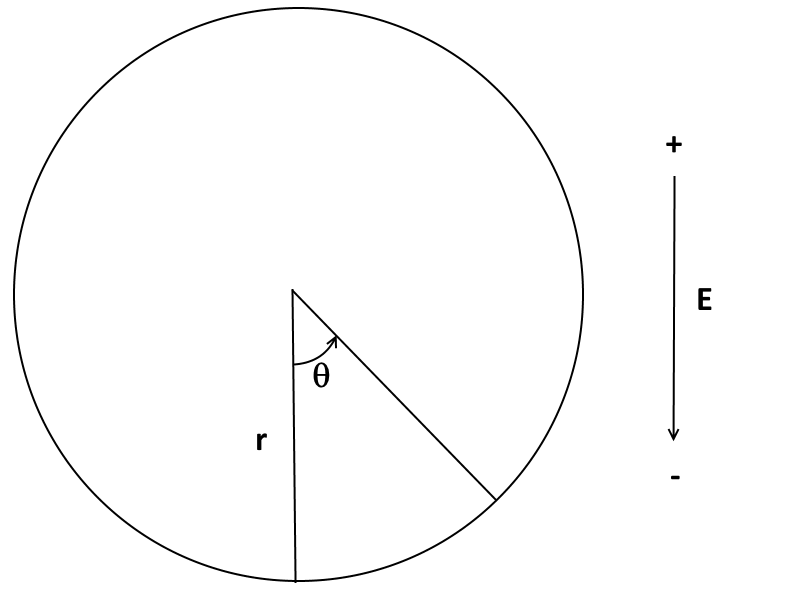
\includegraphics[width=0.40\linewidth]{celula}
%	\caption{PTM en función del tiempo en distintos ángulos polares para dos potenciales aplicados diferentes}
%	\label{fig:itv-time}
%\end{figure}

%\begin{figure}[h]
%\floatbox[{\capbeside\thisfloatsetup{capbesideposition={right,top},capbesidewidth=4cm}}]{figure}[\FBwidth]
%{\caption{A test figure with its caption side by side}\label{fig:test}}
%{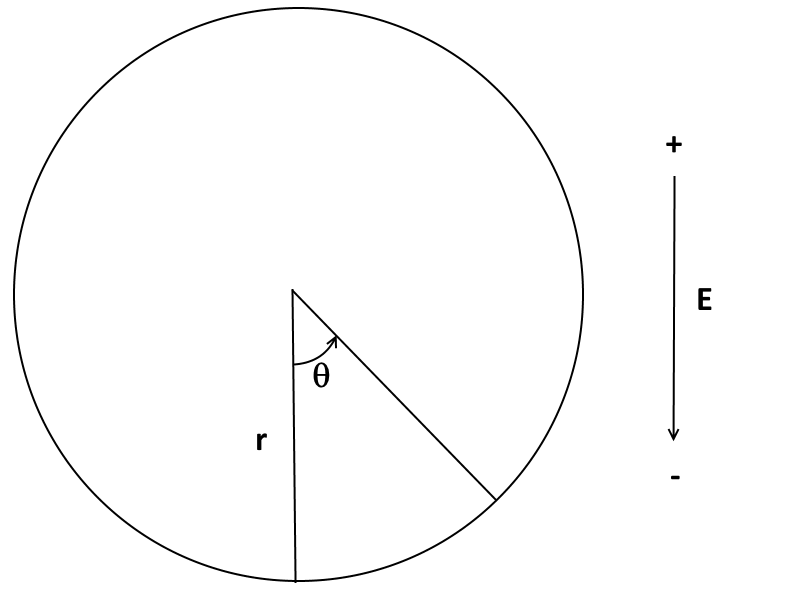
\includegraphics[width=5cm]{celula}}
%\end{figure}

%\begin{figure}[h]
%  \begin{minipage}[r]{0.50\textwidth}
%    \includegraphics[width=\textwidth]{dominio2}
%  \end{minipage}\hfill
%  \begin{minipage}[l]{0.5\textwidth}
%    \caption{
%       Modelo de la célula de radio $r$.\\ $\theta$ representa el ángulo polar\\ y $E$ el campo eléctrico.
%    } \label{fig:03-03}
%  \end{minipage}
%\end{figure}

\begin{figure}[hb]
	\centering
	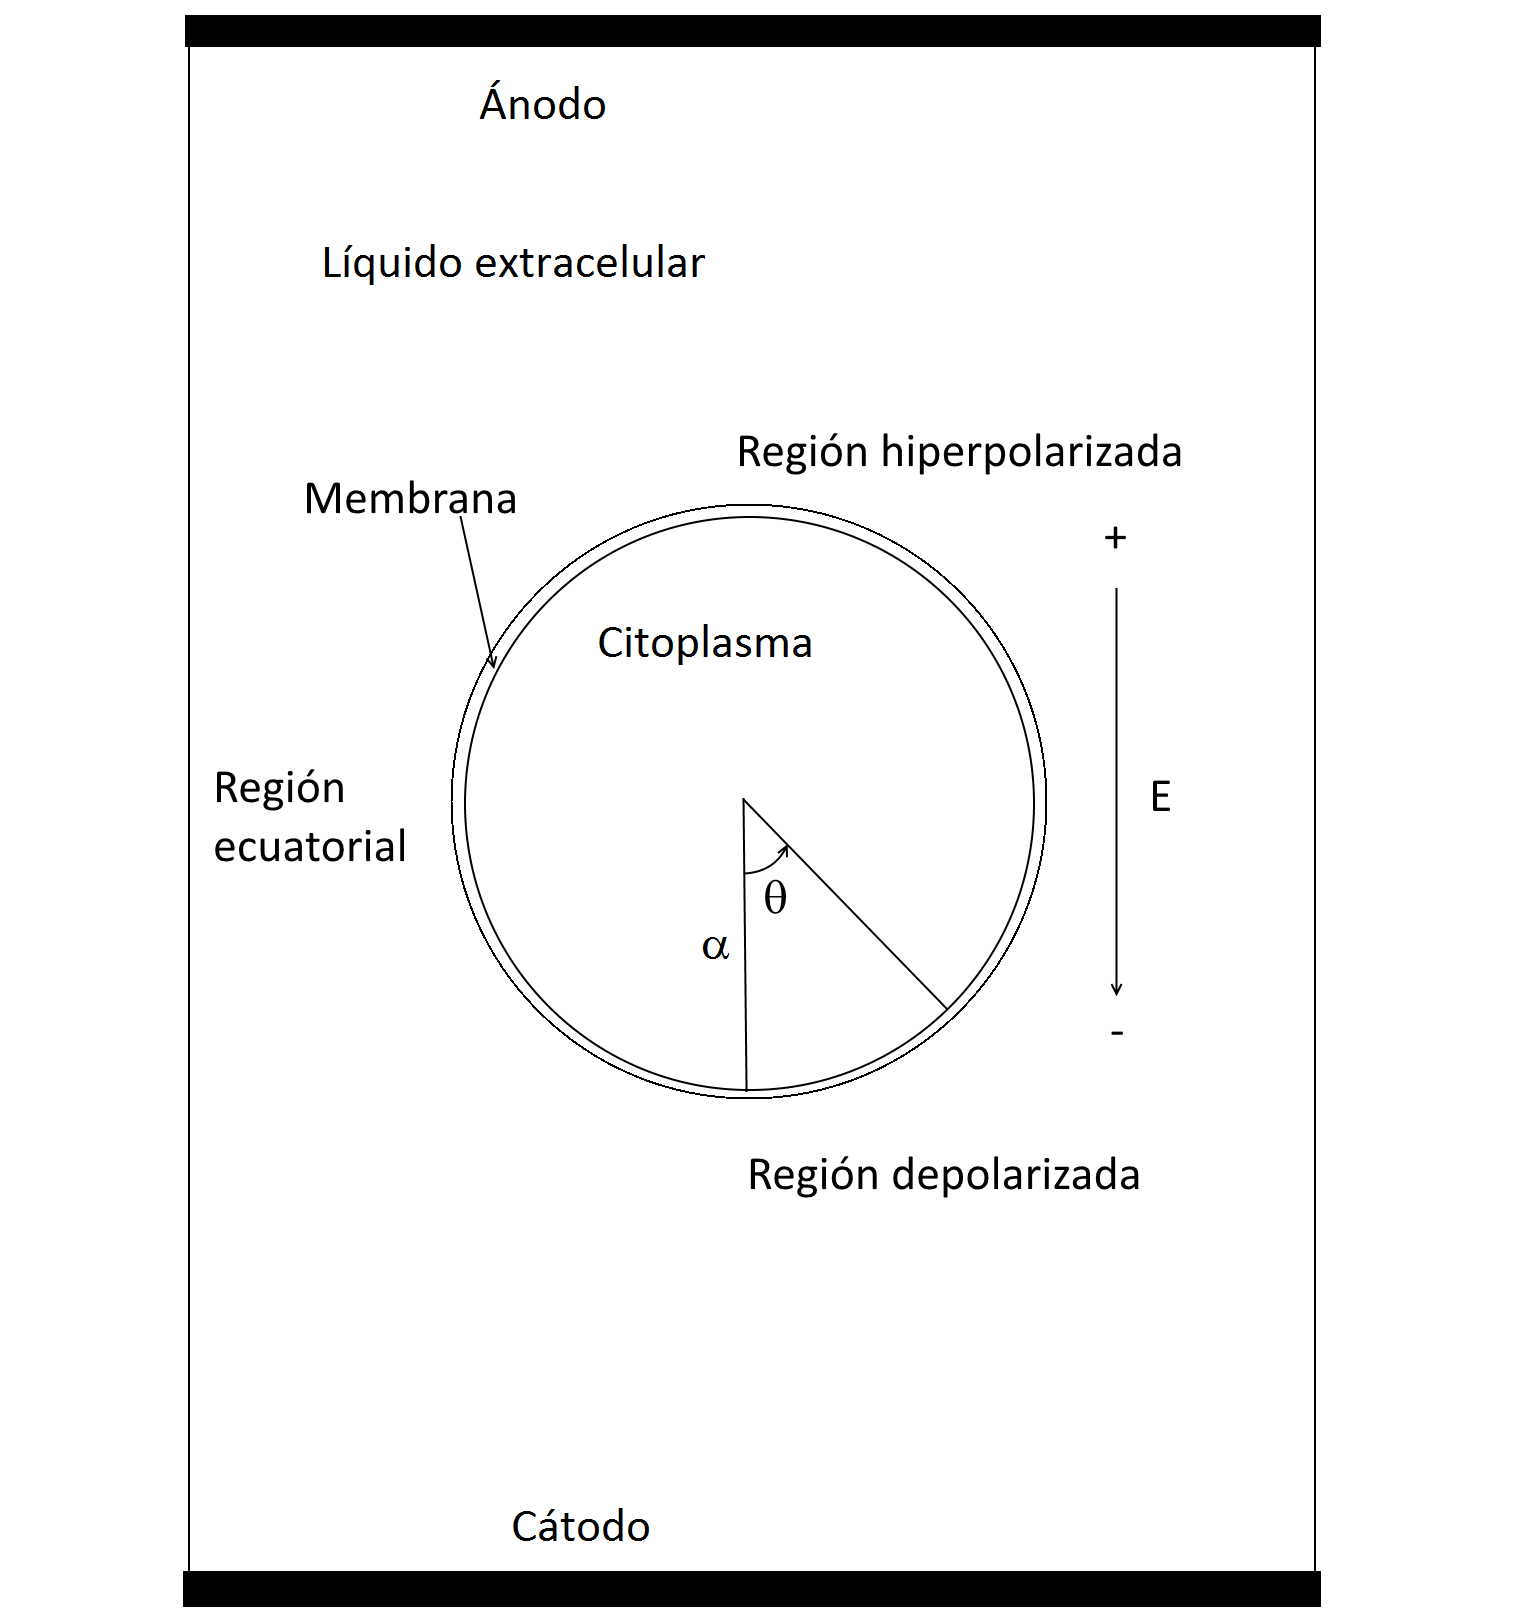
\includegraphics[scale=0.30]{dominio}
	\label{fig:dominio}
	\caption{Dominio del problema}
\end{figure}

\clearpage

Los pulsos se dividen en dos partes con un tiempo de encendido (\ontime) en el que la diferencia de potencial es constante y un tiempo de apagado (\offtime) sin diferencia de potencial entre los electrodos.

\begin{figure}[h]
	\centering
	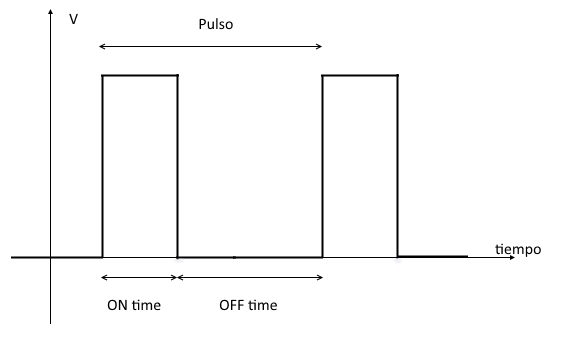
\includegraphics[scale=0.75]{pulso}
\end{figure}


\subsection*{Potencial Eléctrico}
El potencial eléctrico generado por los electrodos se calcula en todo el dominio según la ecuación de Laplace \cite{c9-fem-electro}

\begin{equation} \label{eq:poisson}
	\nabla \sigma_{elem} \cdot (\nabla \phi) = 0 
\end{equation}

donde $\phi$ representa el potencial eléctrico y $\sigma_{elem}$ la conductividad del material, para $elem = o, i$ o $m$ para el líquido extracelular, el citoplasma o la membrana celular respectivamente. Los valores de las conductividades son muy diferentes para los tres tipos de material, siendo en particular la conductividad de la membrana celular mucho menor que la del resto del dominio.

La diferencia de potencial entre el interior y el exterior de la célula en un punto de su superficie se conoce como potencial transmembrana (PTM). Si la célula es esférica este potencial se puede aproximar con la fórmula cerrada \cite{tsong}

\begin{equation} \label{eq:cos}
	 V^{\theta} = f_s\, E\, \alpha\, \cos (\theta) 
\end{equation}

con

\begin{equation} \label{eq:lambda}
    f_s = \frac{3\sigma_o \left( 3 d \alpha^2 \sigma_i + \left( 3 d^2 \alpha - d^3 \right) \left(\sigma_m - \sigma_i \right) \right)}{2 \alpha^3 \left( \sigma_m + 2 \sigma_o \right) \left(\sigma_m + \frac{1}{2} \sigma_i \right) - 2 \left(\alpha - d \right)^3 \left(\sigma_o - \sigma_m \right) \left( \sigma_i - \sigma_m \right)}
\end{equation}

donde $E$ es el campo eléctrico, $\theta$ el ángulo polar respecto del campo eléctrico, $\alpha$ el radio de la célula y $\sigma_o$, $\sigma_i$ y $\sigma_m$ las conductividades del líquido extracelular, intracelular y de la membrana respectivamente. Cuando el valor de $\sigma_m$ es al menos cinco órdenes de magnitud menor que $\sigma_o$ y $\sigma_i$, el valor de $f_s$ se puede aproximar como $3/2$\cite{c5-puchiar}. La fórmula \ref{eq:cos} no tiene en cuenta que el PTM puede variar en el tiempo por la creación de poros, por eso en este trabajo no se la usa directamente, si no que usa la ecuación \ref{eq:poisson}.

\subsection*{Generación y evolución de poros}
El PTM genera en la membrana celular la aparición de poros hidrofílicos, cuya variación de la densidad de poros en el tiempo se puede describir según la ecuación diferencial ordinaria \cite{krass-viejo}

\begin{equation} \label{eq:poros-crea}
	\frac{\partial N}{\partial t} = \alpha_c e^{(V_m/V_{ep})^2} \left( 1 - \frac{N}{N_0 e^{q \left(V_m/V_{ep} \right) ^2}} \right)
\end{equation}

%poner cita \cite{krass}
donde $N$ es la densidad de poros en un determinado tiempo y posición de la membrana celular, $\alpha_c$ es el coeficiente de creación de poros, $V_m$ es el potencial transmembrana, $V_{ep}$ es el voltaje característico de electroporación, $N_0$ es la densidad de poros en equilibrio (cuando $V_m = 0$) y $q$ es una constante igual a $(r_m / r*)^2$, donde $r_m$ es el radio de mínima energía para $V_m = 0$ y $r*$ es el radio mínimo de los poros. Esta ecuación se usa para cada región de la membrana por separado, ya que depende del PTM, que no es constante en la superficie. 

Los poros se crean con un radio inicial $r*$ y su radio varía en el tiempo según el potencial transmembrana de acuerdo a la ecuación diferencial ordinaria \cite{krass07}

\begin{equation} \label{eq:poros-radio}
	\frac{\partial r}{\partial t} = \frac{D}{kT} \left( \frac{V_m^2 F_{max}}{1+r_h / (r+r_a)} + \frac{4 \beta}{r} \left(\frac{r_*}{r}\right)^4 - 2 \pi \gamma + 2 \pi \sigma_{\textrm{\tiny eff}} r\right)
\end{equation}

donde $r$ es el radio de un poro, $D$ es el coeficiente de difusión para los poros, $k$ es la constante de Boltzmann, $T$ la temperatura absoluta, $V_m$ el potencial transmembrana, $F_{max}$ la máxima fuerza eléctrica para $V_m$ de 1V, $r_h$ y $r_a$ son constantes usadas para la velocidad de advección, $\beta$ es la energía de repulsión estérica, $\gamma$ es la energía del perímetro de los poros, y $\sigma_{\textrm{\tiny eff}}$ es la tensión efectiva de la membrana, calculada como

\begin{equation}
	\sigma_{\textrm{\tiny eff}} = 2 \sigma^\prime - \frac{2 \sigma^\prime - \sigma_0}{(1 - A_p / A)^2}
\end{equation}

% puede ir \cite{krass}
donde $\sigma^\prime$ es la tensión de la interfase hidrocarburo-agua, $\sigma_0$ es la tensión de la bicapa sin poros, $A_p$ es la suma de las áreas de todos los poros en la célula, y $A$ es el área de la célula. En la ecuación \ref{eq:poros-radio}, el primer término corresponde a la fuerza eléctrica inducida por el potencial transmembrana, el segundo a la repulsión estérica, el tercero a la tensión de línea que actúa en el perímetro del poro y el cuarto a la tensión superficial de la célula. Se debe analizar el radio de cada poro individualmente y no en conjunto.\\

Por otra parte se asume que la membrana celular se carga como un capacitor y una resistencia en paralelo. De esta manera el potencial transmembrana no aumenta bruscamente al iniciarse el pulso eléctrico, si no que crece de manera paulatina según la ecuación \cite{hibino}

\begin{equation} \label{eq:capacit} \begin{split}
	V_m = V_p\, (1 - e^{-t/\tau}) , \\ \textrm{con } \tau = \alpha\, C_m \left( \frac{1}{\sigma_i} + \frac{1}{2 \sigma_o} \right)
\end{split} \end{equation}

donde $V_m$ es el potencial transmembrana en un punto de la superficie de la célula, $V_p$ es el potencial obtenido por las ecuaciones de potencial eléctrico en ése mismo punto, $t$ es el tiempo transcurrido desde el comienzo del pulso eléctrico, $\alpha$ es el radio de la célula, $C_m$ es la capacitancia superficial de la célula y $\sigma_i$ y $\sigma_o$ las conductancias intra y extracelulares respectivamente.

\subsection*{Transporte de especies}
Se estudia el transporte de cuatro especies iónicas: \h, \oh, \na y \cl{} en el dominio. Para conocer las concentraciones en las diferentes regiones e instantes de tiempo se utiliza la ecuación de conservación de masa de Nernst-Planck \cite{c6-fodava}

%Para conocer la concentración de las especies iónicas se usa la ecuación de conservación de masa de Nernst-Planck \cite{c6-fodava}

\begin{equation} \label{eq:trans}
	\frac{\partial C_i}{\partial t} = \nabla \cdot \left( D_i \nabla C_i + D_i z_i \frac{F}{R T} C_i \nabla \phi \right)
\end{equation}

%\cite{fodava} abajo
donde $C_i$, $D_i$ y $z_i$ representan la concentración, el coeficiente de difusión y la valencia respectivamente de la especie $i$, para $i = $ \h, \oh, \na ó \cl.
$F$ es la constante de Faraday, $R$ la constante de los gases y $T$ la temperatura. 
Esta ecuación tiene en cuenta la difusión de las partículas (con el término $D_i \nabla C_i$) pero también el efecto de migración producto del campo eléctrico (con el término $D_i z_i \frac{F}{R T} C_i \nabla \phi$). 

\subsection*{Condiciones de borde}
Para la ecuación \ref{eq:poisson} se usan condiciones de borde de Dirichlet con potenciales fijos en los electrodos:

\begin{equation}
	\phi_a \; \textrm{para el ánodo y } \phi_c = 0 \; \textrm{para el cátodo}
\end{equation}


mientras que para el borde no ocupado por electrodos se usan condiciones de borde de Neumann:

\begin{equation}
	\frac{\partial \phi}{\partial \mathbf{n}} = 0
\end{equation}

donde $\mathbf{n}$ representa la normal al borde.\\

Para la ecuación de generación de poros \ref{eq:poros-crea} se usa como condición inicial que la membrana no contiene poros, mientras que para la ecuación \ref{eq:poros-radio} se asume que los poros se crean con un radio inicial $r^*$.

Para la ecuación de transporte de especies \ref{eq:trans} se usan como condiciones iniciales las concentraciones descritas en la tabla \ref{table:tablita}: $C_{e, i}^0$ siendo $e =$ $i$ ó $o$ si se refiere a los nodos del interior o del exterior de la célula respectivamente e $i =$ \h, \oh, \na ó \cl{} para la concentración de cada especie. %y $C_{e,i}$ con $e =$ $a$ ó $c$ si es para el ánodo o el cátodo respectivamente.

Como condición de borde en el borde no ocupado por los electrodos se usa

\begin{equation}
	\frac{\partial C_i}{\partial \mathbf{n}} = 0
\end{equation}

%Para los bordes ocupados por los electrodos se usan los valores fijos $C_{e,i}$ descritos anteriormente.

\clearpage
\subsection*{Constantes}
A continuación se presenta la definición y valores de las constantes usadas.

\newcommand{\lineaTabla}[3]{ ${#1}$ & {#3} & {#2} \\ }

\newcommand{\anodo}[3] {
	\lineaTabla{C_{a,{#1}}}{\num{#2} \si{#3}}{Concentración de #1 en el ánodo}
}

\newcommand{\catodo}[3] {
	\lineaTabla{C_{c,{#1}}}{\num{#2} \si{#3}}{Concentración de #1 en el cátodo}
}

\begin{table}[h!]
    \centering
	\begin{tabular}{|l l l|} 
		\hline Símbolo & Definición & Valor \\
		\hline
		\lineaTabla{\sigma_{o}}{0.20 \si{\siemens\per\metre}}{Conductividad de la zona extracelular}
		\lineaTabla{\sigma_{i}}{0.15 \si{\siemens\per\metre}}{Conductividad de la zona intracelular}
		\lineaTabla{\sigma_{m}}{\num{5e-6} \si{\siemens\per\metre}}{Conductividad de la membrana celular}
		\lineaTabla{\sigma_{p}}{2 \si{\siemens\per\metre}}{Conductividad del líquido que llena el poro}
		\lineaTabla{E}{1000\vcm - 2000\vcm}{Campo eléctrico aplicado}
		\lineaTabla{\alpha}{10 \si{\micro\metre} - 50 \si{\micro\metre}}{Radio de la célula}
		\lineaTabla{d}{5 \si{\nano\metre}}{Ancho de la membrana}
		
		\lineaTabla{D_{\h}}{\num{12500} \si{\micro\metre\per\metre^{2}}}{Coeficiente de difusión para \h}
		\lineaTabla{D_{\oh}}{\num{7050} \si{\micro\metre\per\metre^{2}}}{Coeficiente de difusión para \oh}
		\lineaTabla{D_{\na}}{\num{1780} \si{\micro\metre\per\metre^{2}}}{Coeficiente de difusión para \na}
		\lineaTabla{D_{\cl}}{\num{3830} \si{\micro\metre\per\metre^{2}}}{Coeficiente de difusión para \cl}	
		\lineaTabla{C_{i,\h}^0}{\num{.3978e-7} \si{\textsc{m}}}{Concentración inicial de \h{} en citoplasma}
		\lineaTabla{C_{i,\oh}^0}{\num{.3978e-7} \si{\textsc{m}}}{Concentración inicial de \oh{} en citoplasma}
		\lineaTabla{C_{i,\na}^0}{\num{142} \si{\milli\textsc{m}}}{Concentración inicial de \na{} en citoplasma}
		\lineaTabla{C_{i,\cl}^0}{\num{108} \si{\milli\textsc{m}}}{Concentración inicial de \cl{} en citoplasma}

		\lineaTabla{C_{o,\h}^0}{\num{1e-7} \si{\textsc{m}}}{Concentración inicial externa de \h}
		\lineaTabla{C_{o,\oh}^0}{\num{1e-7} \si{\textsc{m}}}{Concentración inicial externa de \oh}
		\lineaTabla{C_{o,\na}^0}{\num{14e-7} \si{\milli\textsc{m}}}{Concentración inicial externa de \na}
		\lineaTabla{C_{o,\cl}^0}{\num{4e-7} \si{\milli\textsc{m}}}{Concentración inicial externa de \cl}
	
	\begin{comment}
		\anodo{\h}{1.5e7}{at.\micro\metre^{-3}} 
		\anodo{\oh}{0}{}
		\anodo{\na}{1e12}{at.\micro\metre^{-3}}
		\anodo{\cl}{0}{}

		\catodo{\h}{0}{}
		\catodo{\oh}{1.806e7}{at.\micro\metre^{-3}}
		\catodo{\na}{0}{}
		\catodo{\cl}{0}{}
	\end{comment}
		
		\lineaTabla{r*}{0.51 \si{\nano\metre}}{Radio mínimo de los poros}
		\lineaTabla{r_m}{0.80 \si{\nano\metre}}{Radio del poro de mínima energía}
		\lineaTabla{\alpha_c}{\num{1e9} \si{\metre^{-2}\siemens^{-1}}}{Coeficiente de creación de poros}
		\lineaTabla{V_{ep}}{0.258 \si{\volt}}{Voltaje característico}
		\lineaTabla{N_0}{\num{1.5e9} \si{\metre^{-2}}}{Densidad de poros en equilibrio}
		\lineaTabla{D}{\num{5e-14} \si{\metre^{-2}\siemens^{-1}}}{Coeficiente de difusión para poros}
		\lineaTabla{F_{max}}{\num{0.7e-3} \si{\newton\volt^{-2}}}{Máxima fuerza eléctrica}
		\lineaTabla{r_h}{\num{0.97e-9} \si{\metre}}{Constante usada para la velocidad de advección}
		\lineaTabla{r_a}{\num{0.31e-9} \si{\metre}}{Constante usada para la velocidad de advección}
		\lineaTabla{\beta}{\num{1.4e19} \si{\joule}}{Repulsión estérica}
		\lineaTabla{\gamma}{\num{1.8e11} \si{\joule\per\metre}}{Energía del perímetro de los poros}
		\lineaTabla{\sigma^\prime}{\num{2e-2} \si{\joule\metre^{-2}}}{Tensión de la interfase hidrocarburo-agua}
		\lineaTabla{\sigma_0}{\num{1e-6} \si{\joule\metre^{-2}}}{Tensión de la bicapa sin poros}
		\lineaTabla{C_m}{\num{1e-14} \si{\farad\metre^{-2}}}{Capacitancia superficial de la célula}

		\lineaTabla{F}{\num{9.648534} \si{\coulomb\per\mole}}{Constante de Faraday}
		\lineaTabla{R}{\num{8.3144621} \si{\joule\per\coulomb\per\mole}}{Constante de los gases}
		\lineaTabla{T}{310 \si{\kelvin}}{Temperatura}
		\lineaTabla{k}{\num{1.3806488e-23} \si{\joule\per\kelvin}}{Constante de Boltzmann}
		
		\hline
	\end{tabular} 
	\caption{Valores constantes usados.Valores obtenidos de  \cite{c4-marino}, \cite{c5-puchiar} y \cite{krass07}}
	\label{table:tablita}
\end{table}

\newpage

\section{Métodos Computacionales}

%Las ecuaciones descritas en la sección anterior fueron resueltas utilizando los métodos numéricos de elementos finitos y diferencias finitas. 

La complejidad de las ecuaciones descritas en la sección anterior obliga a resolverlas con métodos numéricos. Se eligieron los métodos de elementos finitos y diferencias finitas, que fueron totalmente desarrollados en este trabajo. El método de elementos finitos requiere además resolver sistemas de ecuaciones lineales, los cuales se resolvieron utilizando la librería Eigen \cite{eigen}.

\subsection*{Método de Elementos Finitos}

El método de elementos finitos (FEM, \textit{Finite Element Method}) es una herramienta computacional que se utiliza para resolver ecuaciones diferenciales discretizando el dominio en zonas pequeñas llamadas elementos y resolviendo un sistema de ecuaciones lineales con el que se obtiene la solución de las ecuaciones diferenciales en un conjunto de puntos del dominio. Una ventaja del método es que permite modelar con facilidad dominios con formas complejas, y que permite enfocar la atención en zonas del dominio que sean de particular interés, o que contengan cambios bruscos en la solución del problema, modelando sin problemas con elementos de tamaño variable. La aplicación del método de elementos finitos consiste en \cite{zien, gouri}:

\begin{itemize}
	\item Discretizar el dominio continuo en una malla formada por elementos unidos por nodos. Cada uno de estos elementos debe ser pequeño y tener una forma simple (por ejemplo triángulos o cuadriláteros si el dominio es bidimensional). El conjunto de elementos debe ser disjunto y ocupar todo el dominio; es decir, cada punto del dominio debe estar ocupado por uno y sólo un elemento. Los vértices de los elementos se llaman nodos, y suelen ser un punto en común entre dos o más elementos. Cuántos más pequeños sean los elementos, mayor será la precisión de la solución al aplicar el método, pero se necesitarán más elementos para cubrir el dominio, y por lo tanto un mayor poder de cómputo. 

	\item Definir funciones de forma. Una función de forma  de un nodo de un elemento es una función tal que vale 1 cuando se evalúa en el nodo que la define, 0 cuando se evalúa en los demás nodos del elemento, y tiene valores intermedios para los demás puntos del interior. 

	\item Plantear la ecuación $R(e) = \int_{v} N \cdot (L(u) + f_v)\, dv$  para cada elemento, donde la ecuación diferencial a resolver tiene la forma $L(u) + f_v = 0$, $N$ es un vector con las funciones de forma definidas anteriormente, y $R(e)$ es el residuo del elemento, que se intentará minimizar. Luego igualar el residuo a 0 y obtener un sistema de ecuaciones lineales de la forma $K u = f$ donde $K$ es una matriz de $n_e \times n_e$, con $n_e$ la cantidad de nodos por elemento, $u$ es el vector con los valores nodales de la ecuación a resolver y $f$ es un vector de longitud $n_e$. La matriz $K$ del sistema generado se denomina matriz de rigidez, y el vector $f$ vector de fuerza. Para llegar al sistema de ecuaciones lineales suele ser necesario usar integración por partes para reducir el orden de las ecuaciones diferenciales y puede ser necesario resolver integrales con métodos aproximados de integración numérica. La manera de llegar al sistema de ecuaciones lineales depende de la ecuación diferencial a resolver, del tipo de los elementos usados y de las funciones de forma elegidas. 
	
	\item Ensamblar todos los sistemas de ecuaciones elementales en un sistema grande, con tantas ecuaciones e incógnitas como nodos en la malla. El valor en cada nodo debe ser igual para los diferentes elementos a los que pertenece. El proceso de ensamblaje se realiza reescribiendo cada sistema elemental obtenido en el punto anterior por un sistema global, de $n \times n$, donde cada elemento de la matriz de rigidez $K$ se coloca en la posición correspondiente al nodo que representa según la numeración global de los nodos en todo el dominio, y el resto de los elementos se dejan en 0. Luego se suman todas las matrices globales de cada elemento para obtener una única matriz global de rigidez del sistema. Lo mismo se debe realizar con el vector de fuerza $f$. La cantidad de elementos distintos de cero en cada fila $i$ de la matriz de rigidez depende de la cantidad de elementos a los que pertenece el nodo $i$ en la malla que representa el dominio y de la cantidad de nodos por elemento.
	
	\item Agregar las condiciones de borde al sistema global. En algunos casos es posible realizar este paso al generar las ecuaciones elementales, es decir antes de ensamblar el sistema. Diferentes condiciones de borde se agregan de diferentes maneras. Por ejemplo la condición de borde de Dirichlet en un nodo $i$ se puede agregar al sistema reemplazando la fila $i$ de la matriz de rigidez por una fila con 1 en la posición $i$ y ceros en las demás posiciones, y reemplazando el valor en la posición $i$ del vector de fuerza por el valor indicado por la condición de borde. 
	
	\item Resolver el sistema ensamblado con algún método de resolución de ecuaciones lineales. El vector $u$ global obtenido contiene las soluciones en los nodos de la ecuación diferencial. Dado que la matriz ensamblada es muy poco densa (muy pocos elementos distintos de cero), se suele representar con estructuras especiales para matrices dispersas. Si la matriz de rigidez global $K$ es simétrica definida positiva\footnote{$K$ es simétrica definida positiva si $K = K^\intercal$ y $x^\intercal K x > 0$ para todo vector $x \neq 0$} se pueden utilizar métodos especiales como descomposición de Cholesky, LDL o gradientes conjugados, que pueden reducir sustancialmente los tiempos de cómputo. También se pueden reducir los tiempos de resolución si se tiene una matriz banda\footnote{$K$ es una matriz con banda $p$ si $K_{ij} = 0 \; \forall j < i-p$ ó $j > i+p$, es decir todos los valores distintos de cero están dentro de una banda diagonal con un ancho conocido} de rigidez. Para lograr esto último es necesario haber asignado números a los nodos de la malla de manera tal que se minimice la máxima distancia entre los números de dos nodos en un mismo elemento en todo el dominio.\\
\end{itemize}

\newpage

%TODO faltaría fuente de esto}
\subsubsection*{Función de forma bilineal lagrangiana}
En particular en este trabajo se usan elementos cuadrilaterales y funciones de forma lagrangianas bilineales. Para trabajar con facilidad se realiza un cambio de variables que transforma cualquier elemento cuadrilateral en un cuadrado estándar. Esto permite trabajar con las mismas funciones de forma para todos los elementos, aunque estos tengan formas o tamaños muy variados. Esta proyección se conoce como transformación isoparamétrica.\\
	
\setlength{\unitlength}{1cm}
\begin{picture}(10,5)
\put(1,0){\vector(0,1){5}}
\put(0,1){\vector(1,0){5}}
\put(5.2,1.2){$x$}
\put(1.2,4.6){$y$}

\put(1.5,1.5){\circle*{0.15}}
\put(2.5,3.5){\circle*{0.15}}
\put(4.5,4.5){\circle*{0.15}}
\put(4.5,2.5){\circle*{0.15}}

\thicklines
\put(1.5,1.5){\line(1,2){1}}
\put(2.5,3.5){\line(2,1){2}}
\put(4.5,4.5){\line(0,-2){2}}
\put(4.5,2.5){\line(-3,-1){3}}

\put(5, 3){\vector(1,0){1.5}}

\thinlines
\put(7,2.5){\vector(1,0){5}}
\put(9.51,0){\vector(0,1){5}}
\put(12,2.7){$\xi$}
\put(9.7,4.6){$\eta$}

%centro en 9.5, 2.5

\put(8.5,1.5){\circle*{0.15}}
\put(8.5,3.5){\circle*{0.15}}
\put(10.5,1.5){\circle*{0.15}}
\put(10.5,3.5){\circle*{0.15}}

\thicklines
\put(8.5,1.5){\line(0,1){2}}
\put(8.5,3.5){\line(1,0){2}}
\put(10.5,1.5){\line(-1,0){2}}
\put(10.5,3.5){\line(0,-1){2}}

\put(6.5,1.2){$(-1,-1)\; 1$}
\put(7.2,3.7){$(-1, 1)\; 4$}
\put(10.7,1.2){$2 \;(1, -1)$}
\put(10.7,3.7){$3 \;(1, 1)$}

\end{picture}	

La proyección tranforma puntos de las coordenadas reales $(x, y)$ a coordenadas locales $(\xi, \eta)$ en el rango $[-1, 1]$. Las funciones de forma bilineales lagrangianas son:

%\begin{equation}
%    N_i(\xi, \eta) = \frac{1}{4} (1 + \xi_i \, \xi) (1 + \eta_i \, \eta) \;\; \mathrm{para} \; i = 1, \ldots, 4
%\end{equation}

\begin{equation}
    N_i(\xi, \eta) = \frac{1}{4} (1 + \xi_i \, \xi) (1 + \eta_i \, \eta)
\end{equation}

para $i = 1, \ldots, 4$, donde $\xi_i$ y $\eta_i$ son las coordenadas locales del punto $i$ (que valen $-1$ o $1$).  Es fácil ver que la función de interpolación $i$ vale 1 en el punto $(\xi_i, \eta_i)$, 0 en $(\xi_j, \eta_j)$ para $j \neq i$ y valores intermedios para cualquier otro punto del cuadrado estándar. Esta función de forma es una función de interpolación de primer orden y usa únicamente los 4 elementos de las esquinas del cuadrilátero, mientras que otras funciones de forma son polinomios de mayor grado que usan también puntos intermedios del elemento.

\subsubsection*{Integración por cuadratura de Gauss}

Para resolver las integrales necesarias en el método de elementos finitos, se recurrió a la integración numérica. El método de cuadratura de Gauss permite obtener una aproximación de la integral definida de una función en un intervalo evaluando la función a en una serie de puntos y realizando una suma pesada de los valores. En forma general se puede integrar en dos dimensiones en el cuadrado estándar como

\begin{equation}
    \int_{-1}^1 \int_{-1}^{1} f(\xi, \eta) \, \mathrm{d\eta} \, \mathrm{d\xi} \approx \sum_{j=1}^{n} \sum_{i=1}^{n} w_j \, w_i \, f(r_i, r_j)
\end{equation}

donde $n$ es la cantidad de puntos elegidos para realizar la cuadratura, $w_i$ es el peso del iésimo punto y $r_i$ es el iésimo punto. Tanto los $w_i$ como los $r_i$ corresponden a las raíces de los polinomios de Legendre. En el caso particular de esta tesis se trabajó con $n = 2$ puntos, por lo tanto corresponden los siguientes valores: $r_1 = -\sqrt{1/3}, r_2 = \sqrt{1/3}, w_1 = w_2 = 1$.

%TODO podría ir Método de Diferencias Finitas

\subsection*{Descomposición LDL}
La factorización LDL permite descomponer una matriz $A$ simétrica en $A = L D L^\intercal$ donde $L$ es triangular inferior con unos en la diagonal, $D$ es diagonal y $L^\intercal$ es la matriz traspuesta de $L$. De esta manera es posible resolver sistemas de ecuaciones lineales de la forma $Ax = b$ con aproximadamente la mitad de las operaciones que se necesitarían por el método de eliminación gaussiana o LU. Este método puede utilizarse para cualquier matriz $A$ cuadrada simétrica que tenga una descomposición LU sin intercambios de filas. En particular puede aplicarse para todas las matrices simétricas definidas positivas.\\

El algoritmo para obtener las matrices $L$ y $D$ a partir de una matriz $A$ de $n \times n$ es:\\

%\clearpage

\begin{algorithmic}
	\FORALL {$i \in \{1 \ldots n\}$}
		\FORALL {$j \in \{1 \ldots i-1\}$}
			\STATE $v_j = L_{ij} D_{jj}$
		\ENDFOR
		\STATE $D_{jj} = A_{ii} - \Sigma_{j=1}^{i-1} L_{ij} v_j$
		\FORALL {$j \in \{i+1 \ldots n\}$}
			\STATE $L_{ij} = \left( A_{ji} - \Sigma_{k=1}^{j-1} L_{jk} v_k \right) / D_{ii}$
		\ENDFOR
	\ENDFOR
	\RETURN $L, D$
\end{algorithmic}

El algoritmo requiere aproximadamente $\frac{1}{6} n^3 + \frac{1}{2} n^2 - \frac{7}{6}n$
multiplicaciones o divisiones de punto flotante \cite{burden}. La factorización LDL es similar a la descomposición de Cholesky, la cual calcula una descomposición de la forma $A = L'L'^\intercal$, donde $L' = L\sqrt{D}$. Sin embargo el método de Cholesky requiere calcular la raíz cuadrada de la matriz diagonal $D$, lo cual tiene un costo computacional y un error de cálculo adicional. LDL tiene además como ventaja que funciona en algunos casos en los que $A$ no es una matriz definida positiva, lo cual no sucede con la descomposición de Cholesky.
%TODO{se podría hablar de estabilidad}

\subsection*{Descomposición de gradiente biconjugado estabilizado}
El método del gradiente biconjugado estabilizado (BiCGSTAB por \textit{biconjugate gradient stabilized method}) es un algoritmo iterativo que sirve para resolver sistemas de ecuaciones lineales de la forma $Ax=b$. BiCGSTAB es una modificación del método del bigradiente conjugado (BCG) que logra una mayor estabilidad numérica y velocidad de convergencia. A su vez BCG es una generalización del método de gradientes conjugados, modificado para funcionar también con matrices no simétricas pero con baja estabilidad numérica. El pseudocódigo del algoritmo es \cite{yousef, fokkema}: 

\clearpage

\newcommand{\walfa}{\widetilde{\alpha}}
\newcommand{\wsigma}{\widetilde{\sigma}}
\newcommand{\wrcero}{\widetilde{r}_0}

\begin{algorithmic}
	\STATE Elegir valores iniciales de $x_0$ y $\wrcero$
	\STATE $r_0 = b - A x_0$
	\STATE $u_{-1} = w_{-1} = s_{-1} = 0$
	\STATE $\alpha_{-1} = \sigma_{-1} = \walfa_{-1} = \wsigma_{-1} = 1$
	\STATE $k = 0$
	\REPEAT
		\STATE $\rho_k = \left( r_k, \wrcero \right)$
		\STATE $\beta_k = (-1 / \walfa_{k-1}) (\rho_k / \sigma_{k-1})$
		\STATE $w_k = r_k - \beta_k (w_{k-1} - \walfa_{k} c_{k-1})$
		\STATE $c_k = A w_k$
		\STATE $\sigma_k = (c_k, \wrcero)$
		\STATE $\alpha_k = \rho_k / \sigma_k$
		\STATE $s_k = r_k - \alpha_k c_k$
		\STATE $t_k = A s_k$ 
		\STATE $\walfa_{k} = (s_k,t_k) / (t_k, t_k)$
		\STATE $x_{k+1} = x_k + \alpha_k w_k + \walfa_{k} s_k$
		\STATE $r_{k+1} = s_k - \walfa_{k} t_k$
		\STATE $k = k + 1$
	\UNTIL {$x_{k}$ no sea lo suficientemente preciso}
	\RETURN $x_k$
\end{algorithmic}

BiCGSTAB funciona particularmente bien comparado con métodos directos cuando se trabaja con sistemas de ecuaciones muy grandes y esparsos, algo que suele suceder a menudo al aplicar el método de elementos finitos. Dado que es un algoritmo iterativo, necesita un criterio de parada que puede estar dado como una medida de la diferencia entre $b$ y $A x_k$. El valor de $x_0$ usado en la primera iteración se puede elegir de manera arbitraria, y el algoritmo puede converger en muy pocas iteraciones si se elije un valor de $x_0$ muy cercano a la solución del sistema. Por esta razón si se resuelven muchos sistemas de ecuaciones similares, se puede usar la solución final de uno como solución inicial del siguiente. 

\section{Implementación}
El problema fue dividido en tres partes, según los tres fenómenos físicos principales considerados: el potencial eléctrico en el dominio, la evolución de los poros en la membrana celular y el transporte de las especies iónicas. 

El trabajo fue implementado en \texttt{C++}. Se hizo uso de varias funcionalidades nuevas incorporadas al lenguaje en \texttt{C++11}, y de la librería de álgebra lineal \nombre{Eigen} para resolver sistemas de ecuaciones. Las simulaciones fueron realizadas en un equipo con procesador Intel i3 2100 corriendo a 3.10 GHz y 8GB de memoria RAM con sistema operativo Microsoft Windows 7. El código es portable y fue compilado con Microsoft Visual C++ bajo la interfaz Microsoft Visual Studio 2013, pero también fue probado con los compiladores Intel C Compiler para Windows y GCC para Linux.

Para realizar las simulaciones de los problemas de potencial eléctrico y transporte de especies se utilizó el método de elementos finitos, que requiere resolver sistemas de ecuaciones lineales. Las resoluciones de los sistemas de ecuaciones se hicieron con la librería \nombre{Eigen}, usando matrices esparsas y los métodos LDL y gradiente biconjugado estabilizado. Las ecuaciones de densidad y radio de poros se resolvieron por el método de diferencias finitas. %Para acelerar los tiempos de ejecución se usó la interfaz \nombre{OpenMP}, que consiste en directivas para paralelizar código \texttt{C++} en múltiples hilos de ejecución. 

Se usó un sistema de coordenadas cilíndricas idealizando la célula y los electrodos como sólidos de revolución. Se generaron mallas bidimensionales con elementos cuadrilaterales de tamaño variable usando el programa \nombre{Auto-Mesh 2D} \cite{automesh}. Las zonas cercanas a la membrana celular son de mucho interés y contienen cambios bruscos de potencial y concentraciones. Por esta razón se usaron elementos muy pequeños en estas regiones. Se distinguen en la malla tres regiones: el líquido extracelular, el citoplasma (en el interior de la célula) y la membrana celular. A diferencia de otros trabajos anteriores la membrana celular se modela en la malla con elementos propios del tamaño real en vez de considerarse con un ancho superior al real o directamente una condición de borde. El método de elementos finitos fue elegido en lugar de el método de diferencias finitas porque permite crear mallas con elementos de tamaños irregulares y realizar cambios en las mallas empleadas sin modificar el programa que realiza la simulación.

\begin{figure} 
\makebox[\textwidth][c] {
	\centering
	\begin{minipage}{.20\paperwidth}
		\centering
		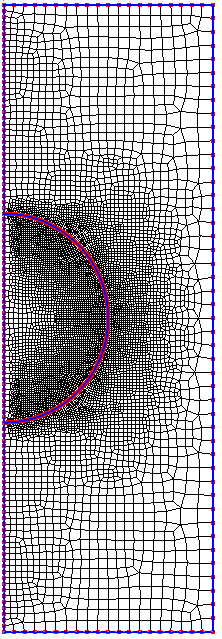
\includegraphics[scale=0.55]{mesh/meshfar}
	\end{minipage}%
	\begin{minipage}{.60\paperwidth}
		%\centering
		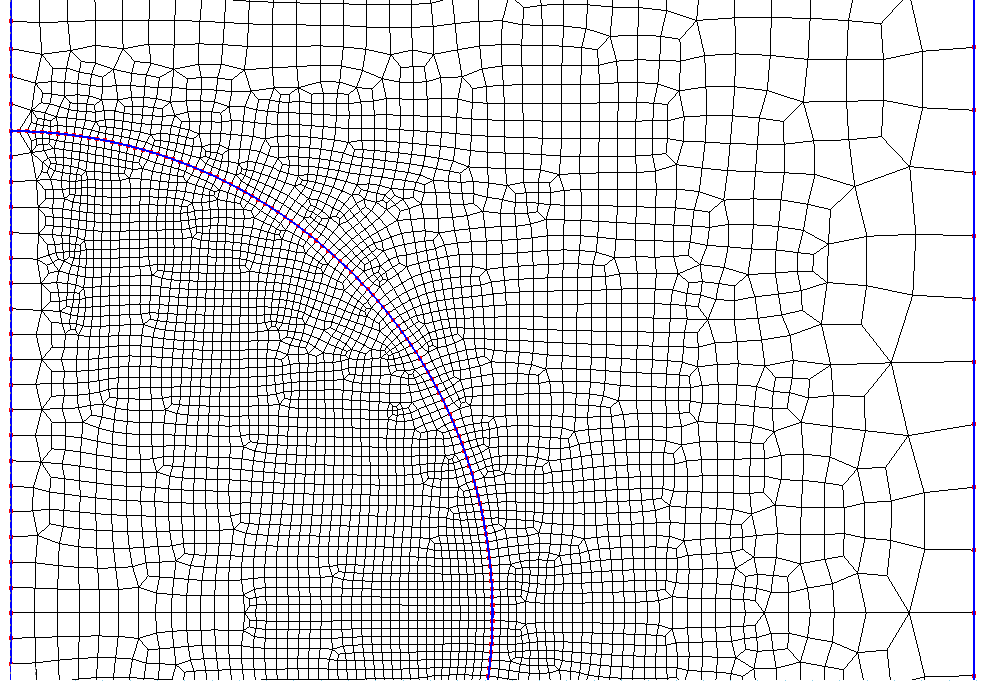
\includegraphics[scale=0.50]{mesh/mesh3}
	\end{minipage}
}
\caption{Ejemplo de malla. Dominio completo (izquierda) y detalle (derecha). La célula tiene forma de semicírculo dado que se usan coordenadas cilíndricas. Los elementos de la membrana son los más pequeños y no se alcanzan a ver.}
\end{figure}


\begin{figure}
	
\includegraphics[width=\textwidth]{mesh/membrana}
	\caption{Detalle de la malla cerca de la membrana. Los líneas dobles corresponden a elementos de la membrana celular, los elementos de la izquierda corresponden al interior de la célula y los de la derecha al exterior.}
	\label{fig:mesh-membrana}
\end{figure}


Las mallas utilizadas tienen entre 7500 y 8900 elementos y representan un dominio de hasta 150 \si{\micro\metre} de alto y hasta 50 \si{\micro\metre} de ancho con una célula cuyo radio varía entre 10 y 50 \si{\micro\metre} y con una membrana de 5 \si{\nano\metre} de espesor. Para modelar la membrana se crearon tres arcos separados a 2.5 \si{\nano\metre} de distancia, que fueron divididos en 192 partes en la dirección del ángulo polar. De esta manera se obtiene una membrana con dos elementos en la dirección radial. Los electrodos se modelaron dentro del dominio, en los bordes superior e inferior.

También se usó \nombre{Python} como lenguaje secundario, para ayudar en la generación de mallas, la interpretación de los datos de salida obtenidos en las simulaciones y la generación de gráficos, haciendo uso de la librería \nombre{matplotlib} \cite{matplotlib}. El programa lee los parámetros de ejecución de un archivo \texttt{input.in} y graba periódicamente resultados de potencial y campo eléctrico, potencial transmembrana, densidad y radios de poros en la membrana celular, concentraciones de las especies y valores de pH en diferentes archivos de salida.

%\clearpage

\subsection*{Escalabilidad}

El código implementado contiene partes que corren en paralelo implementadas con \nombre{OpenMP} para mejorar así los tiempos de ejecución.\\

\textbf{OpenMP} es una API (interfaz de programación de aplicaciones) que permite implementar con facilidad código paralelo con múltiples hilos de ejecución y memoria compartida \cite{quinn}. Consta de un conjunto de directivas para el compilador llamadas \textit{pragmas} y se puede utilizar en programas de Fortran, \texttt{C} y \texttt{C++}. Una de las principales ventajas de \nombre{OpenMP} contra otros paradigmas de paralelización como el pasaje de mensajes, es que con OpenMP es muy fácil convertir código serial a paralelo. Por ejemplo para convertir un ciclo serial que consume mucho tiempo de ejecución a uno paralelo suele bastar con agregar unos pocos \textit{pragmas} al código. Con el modelo de pasaje de mensajes, en cambio, sería necesario reescribir gran parte de la lógica del programa, ya que los diferentes procesos no compartirían memoria y necesitarían enviarse mensajes explícitamente. Como desventaja se tiene que es necesario que todos los núcleos involucrados en el cómputo compartan la misma memoria, lo cual impide utilizar clústers de computadoras limitando la paralelización que es posible obtener. Esto no es un problema en este trabajo, ya que se utilizan mallas bidimensionales relativamente pequeñas y que gran parte del código es serial, y por lo tanto no se obtendría una mejora significativa con una cantidad muy grande de procesos ejecutando en paralelo.\\

%TODO se podría explicar que pragmas se usan en el código

Para medir la mejora obtenida al utilizar varios hilos de ejecución se utilizan las medidas de \textit{speedup} y \textit{eficiencia}. Se define speedup como $S = T_s / T_p$ donde $T_s$ es el tiempo de ejecución serial (con un solo proceso o hilo) y $T_p$ el tiempo de ejecución paralelo \cite{pacheco}. La eficiencia en cambio es $E = S / p$ donde $S$ es el speedup y $p$ la cantidad de procesos o hilos \cite{pacheco}.\\

En la tabla \ref{tab:escala} se encuentran medidas de los tiempos de ejecución, speedup y eficiencia de una simulación similar a las realizadas en el capítulo \ref{chap:acoplado}, usando entre 1 y 4 hilos de ejecución. Se puede ver que los mejores tiempos se obtuvieron con 4 threads, pero sin embargo el speedup es apenas mayor al obtenido con 2 threads, y la eficiencia es mucho menor. Se puede concluir que el programa escala correctamente para 2 threads, pero no mejora notablemente al agregar más hilos de ejecución, e incluso empeora los tiempos de ejecución al pasar de 2 a 3 hilos. La baja escalabilidad puede deberse a que solo una fracción del código corre en paralelo (el armado de matrices del cálculo del potencial eléctrico y el cálculo de las concentraciones de especies), mientras que la mayor parte es serial (los cálculos relacionados a los poros y la factorización de matrices para el potencial eléctrico).

\begin{table}
    \centering
	\begin{tabular}{ c | c c c c }              
		& 1 thread & 2 threads & 3 threads & 4 threads \\
		\hline
		Tiempo [\si{\second}] & 1995 & 1331 & 1489 & 1233 \\
		Speedup & 1 & 1.50 & 1.34 & 1.63 \\
		Eficiencia & 100\% & 74.9\% & 44.7\% & 40.5\% \\
	\end{tabular}
    \caption{Tiempos de ejecución para un pulso de 5 \si{\milli\second} y una malla de 8899 nodos corriendo en un CPU intel i3 2100 a 3.10 GHz con capacidad para 4 threads}
    \label{tab:escala}
\end{table}



\chapter{Potencial Eléctrico}
%% CAP 3 ITV. como se resuelve, resultados (solos, sin poros ni transporte). 
%% Comparar con formula cerrada?

En este capítulo se estudiará el potencial transmembrana generado en una célula por efecto de un pulso eléctrico, usando la ecuación \ref{eq:poisson} descrita en el capítulo anterior. Para eso se presentará el modelo computacional y los resultados serán estudiados. Se estudiará únicamente el potencial eléctrico en el dominio con su campo eléctrico, pero no se tendrá en cuenta la creación de poros en la membrana, los cuales pueden afectar la conductividad de la misma y modificar de esta manera el potencial eléctrico a través del tiempo. 

\section{Implementación}
Para resolver la ecuación \ref{eq:poisson} se utilizó el método de elementos finitos, llenando la matriz de rigidez según los conductividades y coordenadas de los elementos y el vector de masa según las condiciones de borde. La matriz de rigidez generada es simétrica definida positiva y con muy pocos elementos distintos de cero. Por estas razones es representada con una matriz esparsa y el sistema de ecuaciones se resuelve con el método de Cholesky. Una vez resuelto el sistema se obtiene el potencial eléctrico en cada nodo de la malla que representa el dominio. Dado que la creación de la matriz es uno de los pasos con mayor costo computacional, se utiliza \texttt{OpenMP} para llenar la matriz en paralelo, usando tantos threads como sean indicados en el archivo de entrada \texttt{input.in}.

Con los resultados obtenidos por el método de elementos finitos se calcula también el PTM en cada ángulo polar de la célula, comparando los potenciales externos con los internos, habiendo previamente identificado los nodos correspondientes al exterior e interior de cada ángulo discreto. También se calcula el campo eléctrico en el dominio como el gradiente del potencial eléctrico. Los resultados de potencial en el dominio, PTM y campo eléctrico se graban en archivos separados en formato \texttt{.csv}. 

La fórmula cerrada \ref{eq:cos} permitiría obtener con mayor facilidad los potenciales transmembrana sin resolver sistemas de ecuaciones, pero no es utilizada porque no sirve para obtener los potenciales en el resto del dominio, los cuales serán necesarios en capítulos posteriores y porque asume que la conductividad en la membrana es constante, lo cual no será asumido en el capítulo siguiente.

%TODO llenar mucho más en la parte de implementación. detalles de FEM, etc.
%TODO explicar mejor como se calcula el campo!!!

\section{Resultados}
A continuación se presentan los resultados obtenidos de una simulación de una célula de 25\um de radio con dos electrodos que generan un campo eléctrico de 1200\vcm.\\

%\subsection*{Potencial en el dominio}

\newcommand{\dobleimagen}[6]{
	\begin{figure} \centering
		\begin{minipage}{.5\textwidth}
			\centering
			\includegraphics[width=0.9\linewidth]{#1}
			\captionof{figure}{#3}
			\label{fig:#2}
		\end{minipage}%
		\begin{minipage}{.5\textwidth}
			\centering
			\includegraphics[width=0.9\linewidth]{#4}
			\captionof{figure}{#6}
			\label{fig:#5}
		\end{minipage}
	\end{figure}
}

\newcommand{\dobleimagengrande}[6]{
	\begin{figure} 
	\makebox[\textwidth][c] {
		\centering
		\begin{minipage}{.40\paperwidth}
			\centering
			\includegraphics[width=0.9\linewidth]{#1}
			\captionof{figure}{#3}
			\label{fig:#2}
		\end{minipage}%
		\begin{minipage}{.40\paperwidth}
			\centering
			\includegraphics[width=0.9\linewidth]{#4}
			\captionof{figure}{#6}
			\label{fig:#5}
		\end{minipage}
	}
	\end{figure}
}

\dobleimagen{itv/v-close}{itv-pote}{Potencial eléctrico en el dominio}{itv/campo-close}{itv-campo}{Campo eléctrico en el dominio}

%TODO unidad del campo???

\dobleimagengrande{itv/itv-tita}{itv-tita}{PTM en función del  ángulo polar $\theta$\\ según simulación}{itv/itv-cos}{itv-cos}{PTM en función del  ángulo polar $\theta$\\ según fórmula cerrada}


En las figuras \ref{fig:itv-pote} y \ref{fig:itv-campo} se observa el potencial y el módulo del campo eléctrico en el dominio respectivamente. Se observa que el potencial en el interior de la célula es constante y que la diferencia de potencial entre el exterior y el interior varía según la región de la superficie: en las regiones cercanas al ecuador de la célula la diferencia entre el interior y le exterior es casi nula, pero en los polos la diferencia se hace mayor. 
En la figura \ref{fig:itv-tita} se presenta el PTM en función del ángulo polar $\theta$, mientras que en la figura \ref{fig:itv-cos} se graficó la misma diferencia de potencial calculada según la fórmula cerrada \ref{eq:cos}. Como puede observarse, los valores obtenidos con el método de elementos finitos son muy similares a los obtenidos con la fórmula cerrada, lo cual confirma el correcto funcionamiento de la simulación. 

%TODO escribir más...
%TODO mencionar que ITV crece con el radio. Se podrían comparar varias células

% CAP 4 Poros. ecuaciones, como se resuelve, resultados
\chapter{Generación y Evolución de Poros} \label{chap:poros}

En este capítulo se simula la creación de poros en la membrana celular según las ecuaciones \ref{eq:poros-crea} y \ref{eq:poros-radio}. Para eso se utiliza el cálculo del potencial eléctrico realizado en el capítulo anterior, pero se le agrega la ecuación \ref{eq:capacit}, que tiene en cuenta la capacitancia de la célula al momento de calcular el potencial transmembrana y se actualizan los valores de conductividad en la membrana según la permeabilización lograda por los poros.

\section{Implementación}

Como las ecuaciones que gobiernan la creación de poros en la membrana son dependientes del tiempo, fue necesario crear un ciclo que realice iteraciones de las ecuaciones de poros y de potencial eléctrico. La ecuación \ref{eq:poisson} debe correrse periódicamente a pesar de que no depende del tiempo, ya que los valores de conductancias en la membrana ($\sigma_{m}$) son afectados por la aparición de poros. Las ecuaciones \ref{eq:poros-crea} y \ref{eq:poros-radio} fueron discretizadas con el método de Euler a un paso\footnote{Si se tiene una ecuación diferencial ordinaria tal que $Y'(x) = f(x, Y(x))$ y $Y(x_0) = Y_0$, el método de Euler con un paso $h$ aproxima la función $Y$ como $y_0 = Y_0$ y $y_{n+1} = y_n + h\,f(x_n, y_n)$ \cite{kendall}}.

La ecuación \ref{eq:poros-crea} que calcula la densidad de poros en cada región de la membrana fue discretizada como

%TODO esquema implícito, explícito etc!!!

\begin{equation} \label{eq:poros-crea-disc}
	\frac{N_{t+1} - N_{t}}{\Delta t} = \alpha e^{(V_m/V_{ep})^2} \left( 1 - \frac{N_{t}}{N_0 e^{q \left(V_m / V_{ep} \right) ^2}} \right)
\end{equation}

Para obtener el valor de $V_m$ en cada punto de la membrana celular se tienen en cuenta los potenciales obtenidos con el método de elementos finitos y la capacitancia de la célula. Primero se calcula la diferencia de potencial entre los nodos externos e internos de la membrana y luego se aplica la ecuación \ref{eq:capacit} para obtener el PTM real según el tiempo transcurrido desde el comienzo del pulso.

La cantidad de poros en cada región de la membrana se calcula multiplicando la densidad obtenida con la ecuación \ref{eq:poros-crea-disc} por el área de cada región discreta y tomando la parte entera del valor obtenido. El área de cada zona esférica discreta se calcula como 

\begin{equation} \label{eq:area}
	A = 2 \pi \alpha^2 (\cos(\theta_1) - \cos(\theta_2))
\end{equation}

siendo $\alpha$ el radio de la célula y $\theta_1$ y $\theta_2$ los ángulos que delimitan la zona esférica.

Se mantiene para cada zona esférica discreta un vector con cada uno de los poros y sus radios. Si en una iteración la cantidad de poros estimada para una región es mayor a cantidad de poros estimada en la iteración anterior, entonces se agregan poros al vector de la región esférica con radio inicial $r_*$.

Para cada uno de los poros se calcula por separado su radio en cada iteración aplicando la ecuación \ref{eq:poros-radio} discretizada como

\begin{equation} \label{eq:poros-radio-disc}
	\frac{r_{t+1} - r_t}{\Delta t} = \frac{D}{kT} \left( \frac{V_m^2 F_{max}}{1+r_h / (r_t+r_a)} + \frac{4 \beta}{r_t} \left(\frac{r_*}{r_t}\right)^4 - 2 \pi \gamma + 2 \pi \sigma_{\textrm{\tiny eff}} r_t \right)
\end{equation}

Para mejorar los tiempos de ejecución se consideran todos los poros con radio muy pequeño y con cierta antigüedad como iguales en vez de tratarlos individualmente, mientras que a los poros grandes o recién creados se los trata individualmente, aplicando la ecuación \ref{eq:poros-radio-disc} a cada uno, técnica utilizada en \cite{krass07}.

Los valores de conductividad de la membrana son afectados por la aparición de poros. Por esta razón se calcula primero la permeablización de cada región de la membrana como la proporción del área ocupada por poros con la fórmula

\begin{equation} 
    p = \frac{ \sum\limits_{r \in R} \pi r^2 }{A_z}
\end{equation} 

donde $p$ es la permeabilización de una zona esférica de la membrana, $R$ un conjunto con todos los radios de los poros en ésa zona y $A_z$ el área de la zona, calculada según la ecuación \ref{eq:area}. Luego se actualizan los valores de conductividad de cada zona de la membrana como

\begin{equation} 
	\sigma_{\textrm{\tiny elem}} = \sigma_m (1 - p) + \sigma_p p
\end{equation} 

con $\sigma_{\textrm{\tiny elem}}$ la nueva conductividad del elemento finito, $\sigma_m$ la conductividad de la membrana cuando no tiene poros y $\sigma_p$ la conductividad del líquido que llena los poros.

De la misma manera se actualizan los valores de difusión para los elementos de la membrana 

\begin{equation} 
	D{\textrm{\tiny elem}} = D_m (1 - p) + D_p p
\end{equation} 

con $D_m$ la difusión de la membrana celular sin poros y $D_p$ la difusión del líquido que llena los poros. Este cambio en la difusión no tiene por el momento ningún efecto pero lo tendrá en capítulos posteriores cuando se calcule el transporte de especies.

\section{Resultados}

Se corrieron simulaciones con células de 25\um de radio y pulsos de entre 1200\vcm y 1600\vcm y 5 \ms de duración. 

%acá poner histogramas de poros en diferentes instantes. Al menos para dos valores de tensión
%
%4 histogramas en total, para dos valores de tensión

\dobleimagengrandedonde{poros/120kvm/20micro}{histo-120-1}{Distribución de radios de los poros grandes \\ para $E = 1200\,\vcm$ en $t = 20\,\usec$}{poros/120kvm/500micro}{histo-120-2}{Distribución de radios de los poros grandes\\ para $E = 1200\,\vcm$ en $t = 500\,\usec$}{p}

\dobleimagengrandedonde{poros/160kvm/20micro}{histo-160-1}{Distribución de radios de los poros grandes\\ para $E = 1600\,\vcm$ en $t = 20\,\usec$}{poros/160kvm/500micro}{histo-160-2}{Distribución de radios de los poros grandes\\ para $E = 1600\,\vcm$ en $t = 500\,\usec$}{p}

En las figuras \ref{fig:histo-120-1} y \ref{fig:histo-120-2} se presentan histogramas con los radios de los poros grandes creados en diferentes instantes para pulsos de 1200 \si{\kilo\volt\per\centi\metre}. También hay una gran población de poros pequeños (con radio menor a 1 \si{\nano\metre}) que no fueron graficados por ser de poco interés. Se puede observar que la población de poros alcanza valores altos en un primer instante, pero se reduce dramáticamente en los instantes posteriores. En las figuras \ref{fig:histo-160-1} y \ref{fig:histo-160-2} se observa distribución de radios para la misma célula pero con un pulso de 1600 \si{\kilo\volt\per\centi\metre}. Tanto la cantidad como el radio de los poros creados es mayor en el segundo caso, y se observa también una disminución en la población pasados los primeros instantes del pulso. Es importante notar que si bien la cantidad de poros disminuye con el tiempo, los poros que quedan tienen un radio promedio notablemente mayor al de los primeros instantes.

\begin{figure}
	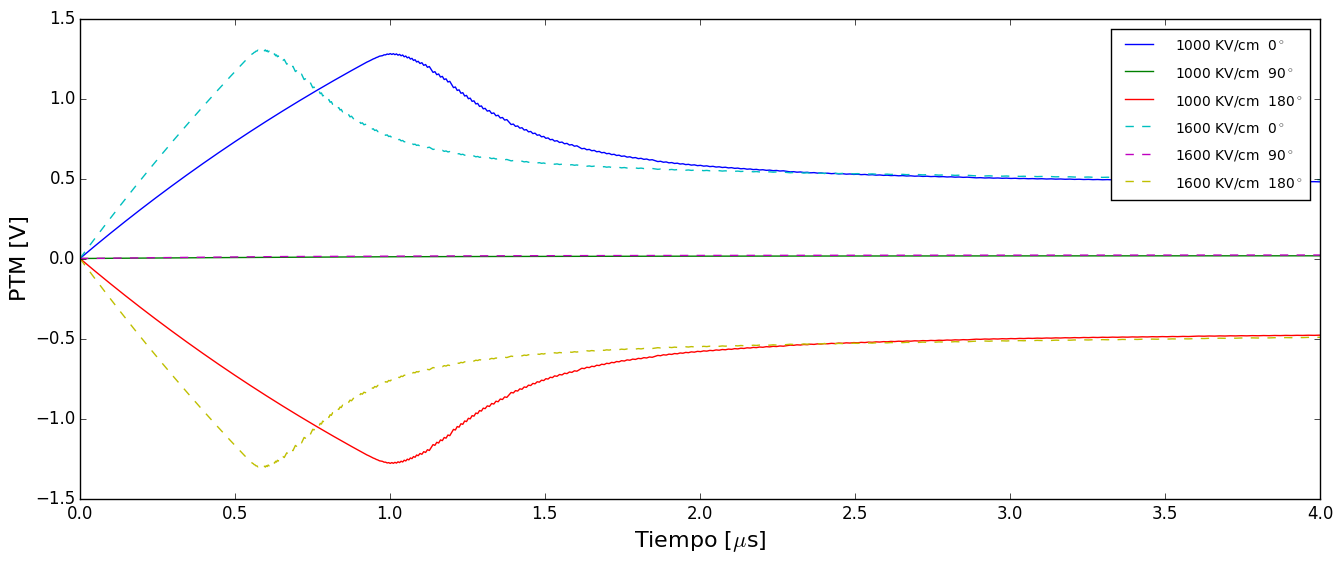
\includegraphics[width=\linewidth]{poros/itv-time}
	\caption{PTM en función del tiempo en distintos ángulos polares para dos potenciales aplicados diferentes}
	\label{fig:itv-time}
\end{figure}

%Se puede observar en la figura \ref{fig:itv-time} el potencial transmembrana en función del tiempo al comienzo del pulso para diferente ángulos polares $\theta$. Las cuatro figuras corresponden a cuatro pulsos de diferente potencial eléctrico aplicado sobre la misma célula. En el primer caso el potencial eléctrico es muy chico y por lo tanto no se alcanzaron a crear poros. En los otros casos el potencial sí es lo suficientemente alto como para crear poros. Se observa en estos casos que el PTM se incrementa durante los primeros instantes hasta alcanzar un pico de tensión a partir del cual comienza a disminuir hasta alcanzar un valor de equilibrio. La subida paulatina de tensión durante los primeros instantes del pulso se debe a la capacitancia de la célula, mientras que la caída en los instantes posteriores se debe a la aparición de poros, que disminuyen la conductividad de la membrana, disminuyendo de esta manera la caída de tensión entre el interior y exterior de la célula. 

%Se nota en todos los casos que las regiones de la membrana cercanas a los polos (con ángulos cercanos a 0º o 180º) obtienen en los primeros instantes los valores absolutos de PTM más altos, mientras que las regiones cercanas al ecuador (ángulo polar cercano a 90º) tienen un PTM prácticamente nulo.

Se puede observar en la figura \ref{fig:itv-time} el potencial transmembrana en función del tiempo al comienzo del pulso para diferentes ángulos polares $\theta$, con dos campos eléctricos diferentes. El PTM se incrementa durante los primeros instantes hasta alcanzar un pico de tensión a partir del cual comienza a disminuir hasta alcanzar un valor de equilibrio. La subida paulatina de tensión durante los primeros instantes del pulso se debe a la capacitancia de la célula, mientras que la caída en los instantes posteriores se debe a la aparición de poros, que disminuyen la conductividad de la membrana, disminuyendo de esta manera la caída de tensión entre el interior y exterior de la célula. Se nota que el PTM obtenido depende notablemente del ángulo polar: en la región polar cercana al electrodo positivo el PTM es positivo y alcanza valores altos, mientras que en el polo cercano al cátodo el potencial es negativo y en el ecuador es cercano a cero. Es llamativo que los valores de campo eléctrico aplicado no influyen en el valor de pico de PTM obtenido, pero si en el tiempo en que éste se alcanza; al aumentar el campo de 1000\vcm a 1600\vcm se acelera el proceso de subida y bajada de PTM hasta alcanzar un equilibrio, pero no se logran aumentar los potenciales obtenidos.


%aca poner gráficos de PTM vs ángulo para diff tiempos. estaría bueno poner una sola curva por gráfico y gráficos más chicos. podrian ser todos de un solo potencial en vez de diferentes tensiones

\dobleimagengrande{poros/120kvm/tita}{tita120}{PTM en función del ángulo polar\\ con $E = 1200\,\vcm$}{poros/160kvm/tita}{tita160}{PTM en función del ángulo polar\\ con $E = 1600\,\vcm$}

En las figuras \ref{fig:tita120} y \ref{fig:tita160} se graficaron los potenciales transmembrana en función del ángulo polar para diferentes instantes de tiempo con pulsos de potenciales diferentes en los dos gráficos. Se observa en los primeros instantes que el PTM obtenido es similar al obtenido en el capítulo anterior y al que se puede estimar con la fórmula cerrada \ref{eq:cos}. Esto se debe a que la población de poros es nula o muy pequeña como para afectar aún la conductividad de la membrana. Sin embargo en los instantes posteriores la aparición de poros disminuye notablemente la conductividad de la membrana en las regiones cercanas a los polos, bajando así la diferencia de potencial. En instantes posteriores se observa el mismo fenómeno con regiones más lejanas a los poros, alejándose más el PTM obtenido del que se puede calcular con la fórmula cerrada \ref{eq:cos}.\\

%%%%

Se estudió también el efecto de aplicar una señal de varios pulsos en lugar uno solo. En la figura \ref{fig:poros-tiempo} se graficó la cantidad de poros en función del tiempo para 4 pulsos de 5\ms de \ontime{} y 5\ms de \offtime{} con varios potenciales diferentes. Se puede ver que la cantidad de poros crece únicamente al principio de cada pulso, y se mantiene casi constante durante el resto del pulso, disminuyendo muy levemente durante el tiempo de apagado. Por cada pulso nuevo se crean poros nuevos, aunque la cantidad de poros nuevos disminuye con cada pulso consecutivo. Se puede ver también que el efecto del campo eléctrico sobre la densidad es enorme, obteniéndose poblaciones de casi el doble de poros para al aumentar el potencial aplicado de 1200\vcm a 1600\vcm. El valor 500\vcm como valor mínimo necesario para obtener una cantidad considerable de poros, mientras que para 400\vcm y otros valores menores la densidad es despreciable, es decir casi no se produce electroporación. 

En la figura \ref{fig:radios-tiempo} se graficó el promedio de los radios de los poros en función del tiempo. Se nota que los radios altos se obtienen por un instante muy corto de tiempo al principio de cada pulso, y que rápidamente se achican llegando a un valor de equilibrio en aproximadamente la mitad del tiempo del \ontime. Cuando el pulso se apaga, los radios se hacen rápidamente mínimos, y se mantienen en un valor muy chico hasta el inicio del próximo pulso. A diferencia de la cantidad de poros, el radio promedio disminuye al aumentar el potencial eléctrico. Esto puede deberse a que un mayor campo eléctrico produce muchos poros de radio mínimo, afectando el promedio de manera negativa. En cada pulso consecutivo parecen aumentar ligeramente los radios obtenidos, notándose la mayor diferencia entre los radios del primer y el segundo pulso. 

En las figuras \ref{fig:pulso1} a \ref{fig:pulso4} se observan las distribuciones de radios de poros para 1600\vcm al instante de 100\usec luego del comienzo de cada pulso. Las diferencias entre radios se observan sobre todo entre el primer y segundo pulso, mientras que los siguientes parecen tener distribuciones muy similares. La mayor concentración se encuentra siempre en los radios muy pequeños (de aproximadamente 1 \si{\nano\metre}), que afectan poco al proceso de permeabilización de la membrana.



\imagensola{poros/poros-tiempo}{poros-tiempo}{Cantidad de poros en función del tiempo para cuatro pulsos}{}
\imagensola{poros/radios-tiempo}{radios-tiempo}{Radio promedio de los poros en función del tiempo para cuatro pulsos}{}



%En las figuras \ref{pulso1} a \ref{pulso4} se observan las distribuciones de radios de poros para cuatro pulsos consecutivos. Los pulsos son de 160\kvcm con 5\ms de \ontime{} y 5\ms de \offtime{} y los histogramas corresponden al instante de 100\usec luego de comenzado cada pulso. \todo[inline]{escribir más después de poner cant poros vs tiempo}

%\dobleimagengrande{poros/160kvm/pulso1}{pulso1}{Primer pulso}{poros/160kvm/pulso2}{pulso2}{Segundo pulso}
%\dobleimagengrande{poros/160kvm/pulso3}{pulso3}{Tercer pulso}{poros/160kvm/pulso4}{pulso4}{Cuarto pulso}

\begin{figure} [ht!]
\makebox[\textwidth][c] {
	\centering
	\begin{minipage}{.43\paperwidth}
		\centering
		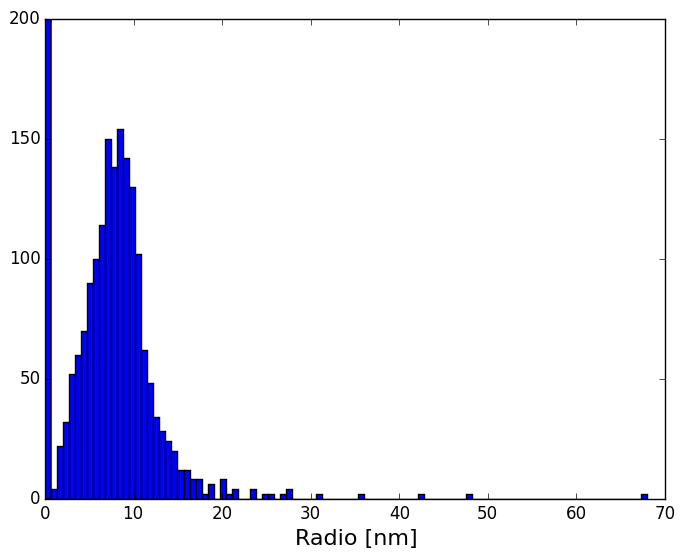
\includegraphics[width=1\linewidth]{poros/160kvm/pulso1}
		\captionof{figure}{Primer pulso}
		\label{fig:pulso1}
	\end{minipage}%
	\begin{minipage}{.43\paperwidth}
		\centering
		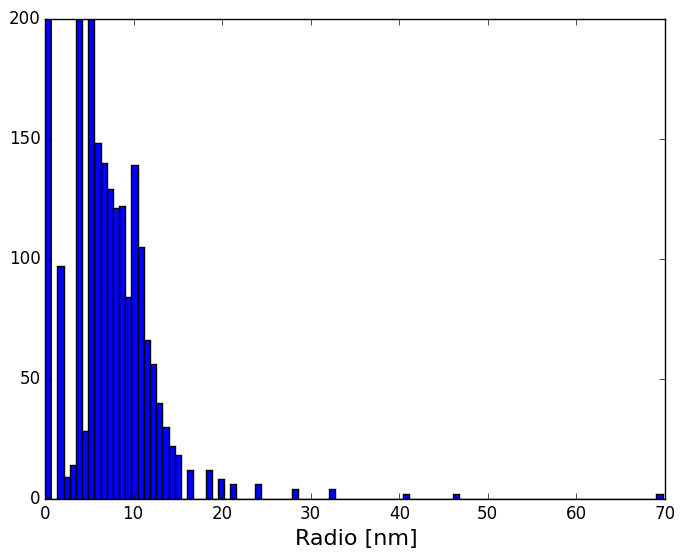
\includegraphics[width=1\linewidth]{poros/160kvm/pulso2}
		\captionof{figure}{Segundo pulso}
		\label{fig:pulso2}
	\end{minipage}
}
\end{figure}

\begin{figure} [ht!]
\makebox[\textwidth][c] {
	\centering
	\begin{minipage}{.43\paperwidth}
		\centering
		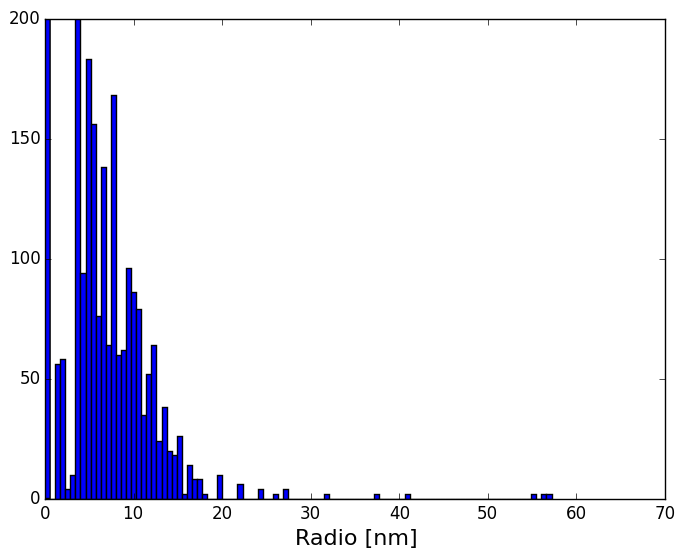
\includegraphics[width=1\linewidth]{poros/160kvm/pulso3}
		\captionof{figure}{Tercer pulso}
		\label{fig:pulso3}
	\end{minipage}%
	\begin{minipage}{.43\paperwidth}
		\centering
		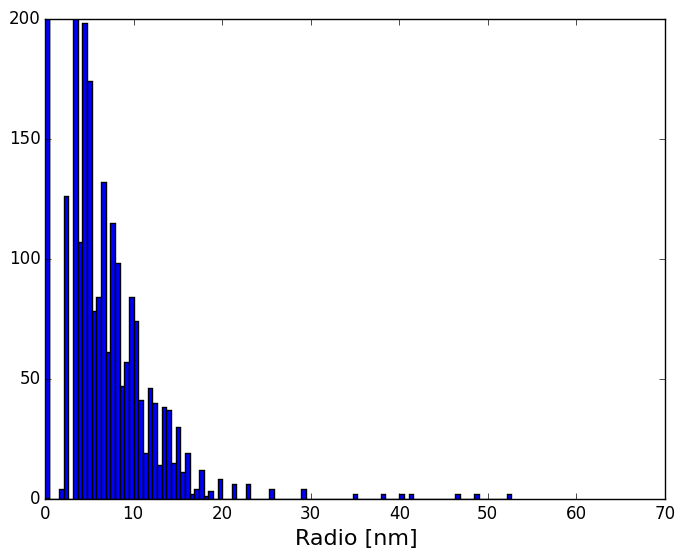
\includegraphics[width=1\linewidth]{poros/160kvm/pulso4}
		\captionof{figure}{Cuarto pulso}
		\label{fig:pulso4}
	\end{minipage}
}
\end{figure}

%TODO conclusiones generales
%TODO mencionar potencial mínimo necesario para electroporación. podría ir tmb un gráfico de itv en tiempo con voltaje bajo sin electroporación
%TODO mencionar que la formula cerrada de itv no sirve


\chapter{Transporte de Especies} \label{chap:trans}
% CAP 5 Transporte. idem (solo transporte, sin poros)

En este capítulo se analiza la concentración y movimiento de distintas especies iónicas en el dominio de la figura \ref{fig:dominio}. \\

Se asume un ánodo de platino, el cual es suficientemente inerte ya que su potencial de reducción es alto. De esta manera es posible despreciar la disolución del metal, siendo así las principales reacciones que se observan: la descomposición del agua y la oxidación de las sustancias ya disueltas en ésta. En el caso de tejidos biológicos, estas reacciones involucran la evolución del oxígeno y cloro, junto a una acidificación, a través de las siguientes reacciones:


\begin{equation}
	\ce{2H_2O <=> O_2 + 4H^+ + 4e^-}
\end{equation}

\begin{equation}
	\ce{2Cl^- <=> Cl_2 + 2e^-}	
\end{equation}

Se asume también un cátodo de platino, siendo la principal reacción catódica la descomposición del agua en hidrógeno molecular e iones hidroxilo:

\begin{equation}
	\ce{2H_2O + 2e^- <=> H_2 + 2OH^-}
\end{equation}

El tejido será considerado como una solución acuosa de cloruro de sodio. Se consideran 4 especies iónicas en el análisis: el hidrógeno (\h), el hidroxilo (\oh), el sodio (\na) y cloruro (\cl). No se considera la capacidad de regulación del tejido. Se realizaron simulaciones en las que se aplicaron pulsos eléctricos y se analizó el transporte de las cuatro especies producto del gradiente de concentración y del campo eléctrico según la ley de Nernst-Planck. No se considera en este capítulo la creación de poros en la membrana celular y su efecto sobre el transporte iónico.

\section{Implementación}

Se utiliza el método de elementos finitos para resolver la ecuación \ref{eq:trans} y obtener las concentraciones de las cuatro especies iónicas en el espacio y el tiempo. Se resuelve primero el potencial eléctrico en el dominio con los métodos usados en el capítulo \ref{chap:itv} y luego se resuelven las concentraciones de masa en diferentes instantes de tiempo.

Las concentraciones de las cuatro especies iónicas se resuelven por separado en un método que genera la matriz de rigidez y el vector de masa para una especie según los resultados de potencial eléctrico, difusión y concentraciones existentes en cada elemento. El sistema de ecuaciones generado se resuelve con el método iterativo de bi-gradientes conjugados estabilizado, dado que la matriz no es simétrica definida positiva. La matriz de masa se representa con una estructura de datos esparsa aprovechando que la mayoría de sus celdas son ceros. Se usa como solución inicial el vector de concentraciones obtenido en la iteración anterior; esto sirve para reducir significativamente la cantidad de iteraciones necesarias para la convergencia del sistema y así reducir los tiempos de ejecución, dado que se espera que en las concentraciones varíen levemente en cada iteración. Las concentraciones de las cuatro especies iónicas se pueden calcular en paralelo en cada iteración, ya que están acopladas entre sí por el campo eléctrico, pero no dependen directamente una de otra. Por esta razón se hace uso de la interfaz \texttt{OpenMP} para realizar las iteraciones de elementos finitos en paralelo usando hasta 4 threads, acelerando así los tiempos de ejecución.

Las concentraciones obtenidas se graban en archivos de salida individuales en intervalos de tiempo fijos usando un formato \texttt{.csv}. Se graban las densidades como cantidad de partículas en unidad de volumen y como concentraciones molares, y también se graban los valores de pH y pOH según las concentraciones de \h y \oh. 

%TODO falta explicar el tema del error de transporte. Faltaría alguna referencia para la fórmula
%TODO se podría mencionar lo de los valores extremos y el truco de subir la temperatura
%TODO explcar concentraciones iniciales?

\section{Resultados}

Se corrió una simulación de un pulso de 100\vcm aplicado sobre una célula de 25\um de radio y se observaron las concentraciones de las cuatro especies iónicas estudiadas. A continuación se presentan los resultados. Debido a que en este capítulo no se tuvo en cuenta la creación de poros en la membrana como en el capítulo anterior, se eligió una diferencia de potencial baja, ya que los valores de potencial transmembrana se vuelven de otra manera muy altos al no haber poros, lo cual originaría concentraciones extremas cerca de la membrana celular en caso de simular campos eléctricos más grandes.

\dobleimagengrande{trans/h}{trans-h}{Concentración molar de \h}{trans/oh}{trans-oh}{Concentración molar de \oh}

\dobleimagengrande{trans/na}{trans-na}{Concentración molar de \na}{trans/cl}{trans-cl}{Concentración molar de \cl}

Las cuatro imágenes de las figuras \ref{fig:trans-h} a \ref{fig:trans-cl} corresponden a concentraciones molares de las cuatro especies estudiadas en el instante $t = 380 \, \si{\micro\second}$ del comienzo del pulso. Se observa en todos los casos extremos altos y bajos de concentraciones en las regiones cercanas a la membrana celular, tanto del lado interno como externo, y valores prácticamente iguales a los iniciales en el resto del dominio, tanto interno como externo a la célula. También se nota que las regiones cercanas al ecuador de la membrana no poseen valores altos ni bajos de concentración, a diferencia del resto de la membrana. Tanto el \h{} como el \na, ambos de carga positiva, logran concentraciones altas en las zonas cercanas al interior de la membrana en el hemisferio depolarizado, y en las zonas cercanas al exterior de la membrana en el hemisferio hiperpolarizado, mientras que alcanzan extremos bajos de concentración cerca del exterior de la membrana en el hemisferio depolarizado y cerca del interior en el hemisferio hiperpolarizado. Las concentraciones de \oh{} y \cl{} --de carga negativa-- se comportan en cambio de manera opuesta, con extremos altos en el interior de la membrana en la región hiperpolarizada y el exterior de la depolarizada y extremos bajos en los otros casos. 

Los cambios en concentración cercanos a la membrana celular se pueden ver en más detalle en las imágenes \ref{fig:curva-h} a \ref{fig:curva-cl}, en las que se analizaron las concentraciones en un corte paralelo al eje de rotación ($z$), que atraviesa la célula por los polos. El ánodo se encuentra en el extremo derecho y el cátodo en el izquierdo, y las líneas punteadas representan la membrana celular. Se ve claramente que los extremos bajos o altos de concentración se dan únicamente en las zonas muy cercanas a la membrana del lado interior o exterior según la carga de la especie y el polo de la célula.\\

%Esto serían como conclusiones
Los resultados obtenidos en este capítulo indican únicamente valores extremos de concentración cerca de la membrana, con diferencias de potencial en los electrodos muy bajas, y muy pocos cambios en el resto del dominio. Este comportamiento se debe a que los valores altos de potencial transmembrana se mantienen en el tiempo, en lugar de disminuir rápidamente como sucedería en la realidad por efecto de la permeabilización de la membrana. En el próximos capítulo se tendrá en cuenta este efecto, y por lo tanto se obtendrán resultados que se acercan mucho más a la realidad.

%TODO{explicar porqué sucede eso}
%TODO{las imágenes pueden ser más interesantes con voltajes mas altos, aunque tenga mucho error}

\imagensola{trans/H-38}{curva-h}{Concentración molar de \h{} en un corte sobre la coordenada $r = 2.5$ \si{\micro\metre}}{1}
\imagensola{trans/OH-38}{curva-oh}{Concentración molar de \oh{} en un corte sobre la coordenada $r = 2.5$ \si{\micro\metre}}{1}

\clearpage %SACAR ESTE CLEARPAGE SI ES NECESARIO!!

\imagensola{trans/Na-38}{curva-na}{Concentración molar de \na{} en un corte sobre la coordenada $r = 2.5$ \si{\micro\metre}}{1}
\imagensola{trans/Cl-38}{curva-cl}{Concentración molar de \cl{} en un corte sobre la coordenada $r = 2.5$ \si{\micro\metre}}{1}


\chapter{Modelo Acoplado} \label{chap:acoplado}
% CAP 6 Todo acoplado. Resultados. poner snapshots de valores 1-9

En este capítulo se realizan simulaciones de todos los fenómenos físicos simulados en los capítulos anteriores juntos, es decir el potencial eléctrico, la creación de poros en la membrana y la posterior variación en el radio de los mismos, las variaciones en la conductividad y difusión de la membrana producto de la aparición de poros y el transporte de especies iónicas en el dominio. Además se estudió el efecto de aplicar varios pulsos consecutivos a través de los electrodos, en lugar de un único pulso.

\section{Implementación}
Para realizar la simulación completa se creó un ciclo principal que realiza llamados a las diferentes rutinas implementadas en los capítulos anteriores.

Para acelerar los tiempos de ejecución se usaron intervalos temporales diferentes para los distintos fenómenos físicos simulados. Para el cálculo de la densidad y radios de los poros en la membrana celular se utilizó un intervalo temporal fijo de 1 \si{\nano\second}, ya que se notó que al aumentarlo se producen errores de discretización muy grandes que derivan en la divergencia del sistema. El cálculo del potencial eléctrico fue realizado periódicamente, a diferencia del capítulo anterior, ya que la aparición de poros afecta los valores de conductividad en la membrana y por consiguiente los potenciales eléctricos en todo el dominio. El intervalo temporal para el potencial eléctrico se eligió dinámico, con valores muy chicos al comienzo del pulso, que se hacen cada ves mayores con el paso del tiempo. Esto es porque se notó que es al principio del los pulsos que se producen cambios muy bruscos en las conductividades de la membrana celular y por lo tanto cambios en el potencial eléctrico que se deben calcular con precisión, pero que luego de un tiempo se alcanzan valores de equilibrio que no requieren intervalos temporales tan pequeños. Exactamente el intervalo temporal para el potencial eléctrico se calcula como

\begin{equation}
	\Delta_t = \mathrm{m_p} \left( 1 - e^{t/k} \right)
\end{equation}

donde $\mathrm{m_p}$ es el máximo valor de intervalo temporal posible, $t$ es el tiempo desde el inicio del último pulso y $k$ es una constante que controla la velocidad con la que aumenta el intervalo temporal. En particular se utilizaron los valores de $\mathrm{m_p} = 2$ \si{\micro\second} y $k = \frac{500 \si{\micro\second}}{\ln (1 - 0.9)}$ para que el intervalo temporal aumente hacia 2 \si{\micro\second} de manera asintótica y alcance el 90\% de este valor en el instante de 500 \si{\micro\second} de comenzado el pulso. En la figura \ref{fig:deltat} se muestra el intervalo temporal en el inicio del pulso. Es importante aclarar que al comenzar y terminar cada pulso se reinicia el cálculo del intervalo temporal.

Por último se utiliza para el cálculo del transporte de especies un intervalo temporal fijo de 200 \si{\nano\second}.\\

\clearpage

\begin{figure}
	\centering
	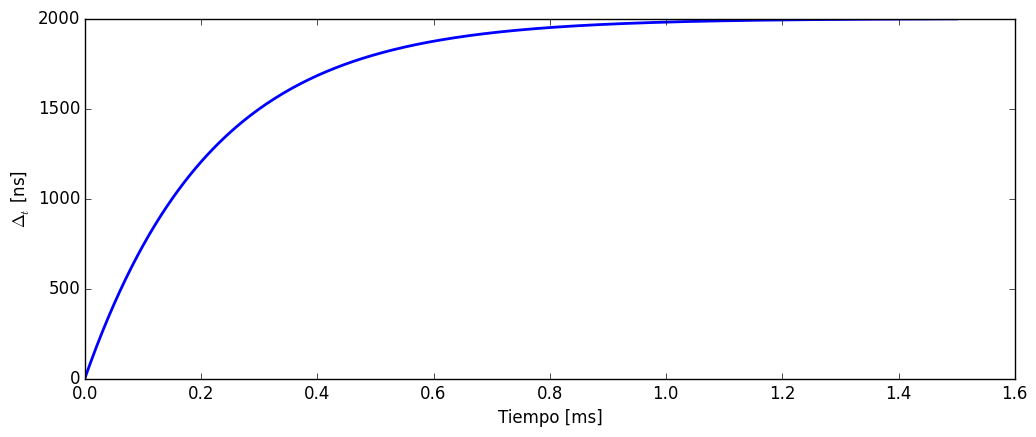
\includegraphics[width=0.8\textwidth]{acoplado/deltat}
	\caption{Intervalo temporal para cálculo del potencial eléctrico en función del tiempo desde el inicio del último pulso}
	\label{fig:deltat}
\end{figure}



% está en este capítulo aunque debería ir en poros!

%Para acelerar los tiempos de ejecución se usaron intervalos temporales diferentes para los distintos fenómenos físicos simulados. Para el cálculo de la densidad de poros en la membrana celular y sus radios se utilizó un intervalo temporal muy pequeño, ya que se notó que al aumentarlo se producen errores de discretización muy grandes que producen la divergencia del sistema. Para el cálculo de los potenciales eléctricos en el dominio, en cambio, alcanzó un intervalo temporal mucho mayor, y se notó que reducirlo no impacta en los resultados. Por último para el cálculo de las concentraciones de las especies iónicas se necesitaron intervalos temporales aún mayores. Concretamente se usaron intervalos de 1 \si{\nano\second} para las ecuaciones de poros, 20 \si{\nano\second} para el transporte de especies y un intervalo variable de entre 1 \si{\nano\second} y 2 \si{\micro\second} para el cálculo del potencial eléctrico. Este último intervalo es variable dado que los primeros instantes de cada pulso eléctrico es el que tiene mayores variaciones en los potenciales producto de la repentina permeabilización de la membrana, como puede verse en el capítulo 4. Esto hace que se necesite una actualización constante de los valores de potencial en los nodos, sobre todos los cercanos a la membrana celular. Sin embargo pasados los primeros microsegundos del pulso el sistema se estabiliza y la permeabilización y valores de PTM se mantienen con pocos cambios lo que hace innecesario un cálculo constante de los potenciales. Por esta razón se optó por un intervalo muy pequeño al comenzar un pulso y se incrementa de manera exponencial.\\

A continuación se presenta el pseudo-código del loop principal del programa. \texttt{nPulsos} es la cantidad de pulsos a simular y $\mathrm{m_p}$, $\mathrm{m_t}$ y $\mathrm{m_d}$ son constantes usadas para determinar los intervalos temporales para el cálculo de potencial eléctrico, el transporte de especies y para grabar los resultados a disco respectivamente.\\


\newcommand{\nextpoiss}{\mathtt{next}_{\mathtt{p}}}
\newcommand{\nextt}{\mathtt{next}_{\mathtt{t}}}
\newcommand{\nextd}{\mathtt{next}_{\mathtt{d}}}

\begin{algorithmic}
	\FORALL{\texttt{pulso} $\in \{1,\ldots, \mathtt{nPulsos}\}$} 
		\FORALL{\texttt{estado} $\in \{\mathtt{ON},\mathtt{OFF}\}$} 
			\STATE $t = 0$
			\STATE $\nextpoiss = \nextt = \nextd = 0$
			\WHILE{$t < \mathtt{duracion[estado]}$} 
				
				\IF{$t \geq \nextpoiss$}
					\STATE calcular potencial eléctrico con \texttt{estado}
					\STATE $\nextpoiss = t + \Delta_t \, \mathrm{m_p} \left(1 - e^{t/k}\right)$
				\ENDIF
				
				\STATE calcular densidad de poros
				\STATE calcular radios de poros
				\STATE actualizar valores de conductividad y difusión
			
				\IF{$t \geq \nextt$}
					\FORALL{$e \in \{$\h, \oh, \na, \cl$\}$} 
						\STATE calcular concentraciones de especie $e$
					\ENDFOR
					
					\STATE $\nextt = t + \Delta_t \, \mathrm{m_t}$
				\ENDIF
				
				\IF{$t \geq \nextd$}
					\STATE grabar estado en disco
					\STATE $\nextd = t + \Delta_t \, \mathrm{m_d}$
				\ENDIF								
				
				\STATE{$t = t + \Delta_t$}
			\ENDWHILE
		\ENDFOR
	\ENDFOR
\end{algorithmic}














%TODO revisar los valores de los intervalos!! revisar si transporte efectivamente mayor que poisson
%TODO mencionar truco numérico temperatura

\section{Resultados}

\subsection*{Un pulso}

\newcommand{\lineasnap}[7]{
	#2 &
	\includegraphics[width=0.19\textwidth]{#1#3.png} & 
	\includegraphics[width=0.19\textwidth]{#1#4.png} & 
	\includegraphics[width=0.19\textwidth]{#1#5.png} & 
	\includegraphics[width=0.19\textwidth]{#1#6.png} & 
	\includegraphics[width=0.19\textwidth]{#1#7.png} \\
}

Se presentan en la tabla \ref{tbl:snap1} las concentraciones en el dominio de las diferentes especies iónicas estudiadas para diferentes instantes de tiempo. Los resultados corresponden a simulaciones de una célula de 25\usec de radio bajo un pulsos eléctrico que genera un campo de 1600\vcm y una duración de 5 \si{\milli\second}. Las imágenes de la tabla \ref{tbl:snap1} corresponden a las concentraciones molares de las cuatro especies en diferentes instantes del pulso. Los colores azules corresponden a los extremos bajos de concentración y los rojos a los extremos altos.

Se observan en todos los casos cambios en el interior de la célula mucho mayores a los obtenidos en las simulaciones del capítulo \ref{chap:trans}. Esto se debe a que la simulación de la generación de poros posibilitó la permeabilización de la membrana y el ingreso o egreso con mayor facilidad de las especies iónicas. 

En el caso del \h{} se observa un gran movimiento en las concentraciones, obteniéndose valores muy altos de concentración en la región hiperpolarizada del interior de la célula, que se observan con una franja roja cercana a la membrana. En cuanto a la región depolarizada del interior, la concentración de \h{} disminuyó notablemente, lo que se observa con una mancha de color verde que avanza hacia el ecuador de la célula con el paso del tiempo. El líquido extracelular también tuvo grandes cambios, con concentraciones altas en la región depolarizada y bajas en la región hiperpolarizada (al contrario del interior).

Las concentraciones de \oh{} presentan un comportamiento opuesto al observado en el \h{}, es decir en el interior de la célula se producen extremos altos de concentración en el polo depolarizado y una disminución de materia en el polo hiperpolarizado, mientras que en el exterior se alcanzan extremos altos cerca de la región de la membrana cercana al polo positivo y extremos bajos en el polo negativo. 

En cuanto a las concentraciones de \na{} y \cl, se observa mucho menos movimiento, dado que sus constantes de difusión son mucho menores que las del \h{} y \oh. Al igual que en los casos anteriores se tienen concentraciones extremas cerca de la membrana, con el mismo patrón de comportamiento según el signo de la especia iónica (el \na{} se comporta como el \h{} por ser de carga positiva y el \cl{} como el \oh{} por ser de carga negativa). No se observa, sin embargo, una zona de concentraciones bajas que avance hacia el centro de la célula, como en los casos anteriores, pero se alcanza a notar que las zonas con valores extremos son de mayor tamaño que las obtenidas en el capítulo \ref{chap:trans}, en el que no se tenía en cuenta la permeabilización de la membrana.

Si bien se observan cambios significativos en las concentraciones de las especies en el interior de la célula, estos cambios se dan principalmente en las regiones cercanas a la membrana. Sin embargo se observa que con el paso del tiempo las regiones con valores extremos se vuelven mayores, lo cuál indica que se podrían obtener mayores cambios en las concentraciones internas con pulsos de mayor duración o con varios pulsos. 

\begin{table}[h!] \begin{center} 
	\begin{tabular}
		{ m{0.5cm} >{\centering\arraybackslash}m{0.17\textwidth} >{\centering\arraybackslash}m{0.17\textwidth} >{\centering\arraybackslash}m{0.17\textwidth} >{\centering\arraybackslash}m{0.17\textwidth} >{\centering\arraybackslash}m{0.17\textwidth} }
		& 1\ms & 2\ms & 3\ms & 4\ms & 5\ms \\
		\lineasnap{acoplado/1p160kvm/h} {\h} {10}{20}{30}{40}{50}
		\lineasnap{acoplado/1p160kvm/oh}{\oh}{10}{20}{30}{40}{50}
		\lineasnap{acoplado/1p160kvm/na}{\na}{10}{20}{30}{40}{50}
		\lineasnap{acoplado/1p160kvm/cl}{\cl}{10}{20}{30}{40}{50}
	\end{tabular}
	\caption{Concentraciones en diferentes instantes de tiempo}
	\label{tbl:snap1}
\end{center} \end{table}

\clearpage

\subsection*{Varios pulsos}

En la tabla \ref{tbl:snap2} se presentan resultados de una simulación similar a la anterior pero con 4 pulsos de 5\ms cada uno, con un tiempo de apagado de 5\ms luego de cada pulso, en lugar de uno solo. Se utilizó la misma célula (de 25\um de radio) y el mismo potencial (1600 \si{\volt\per\centi\metre}). En todos los casos se lograron movimientos de las especies mucho mayores a los obtenidos con un solo pulso. \\

\begin{table} \begin{center} 
	\begin{tabular}
		{ m{0.5cm} >{\centering\arraybackslash}m{0.17\textwidth} >{\centering\arraybackslash}m{0.17\textwidth} >{\centering\arraybackslash}m{0.17\textwidth} >{\centering\arraybackslash}m{0.17\textwidth} >{\centering\arraybackslash}m{0.17\textwidth} }
		& 8\ms & 16\ms & 24\ms & 32\ms & 40\ms \\
		\lineasnap{acoplado/pulsos/h000} {\h} {1}{2}{3}{4}{5}
		\lineasnap{acoplado/pulsos/oh000}{\oh}{1}{2}{3}{4}{5}
		\lineasnap{acoplado/pulsos/na000}{\na}{1}{2}{3}{4}{5}
		\lineasnap{acoplado/pulsos/cl000}{\cl}{1}{2}{3}{4}{5}
	\end{tabular}
	\caption{Concentraciones en diferentes instantes de tiempo}
	\label{tbl:snap2}
\end{center} \end{table}

En las cuatro especies estudiadas se obtuvo lo siguiente:

\begin{itemize}
	\item En el interior de la célula: en todos los casos en los momentos en los que el pulso está encendido se concentran extremos altos de densidad de las especies cerca de la membrana en el hemisferio del mismo signo que la especie (es decir \h{} y \oh{} se concentran en el hemisferio hiperpolarizado y \na y \cl en el depolarizado), mientras que en el polo de signo opuesto se crea una zona con concentraciones bajas que avanzan hacia el ecuador. En cambio cuando el pulso está apagado los valores altos de concentración se dispersan desde la zona cercana a la membrana hacia el interior de la célula, aumentando así la región ocupada por concentraciones altas, mientras que la zona con concentraciones bajas deja de avanzar.

	\item En el exterior de la célula: se crea una zona de concentración alta que rodea la célula empezando en el polo de signo opuesto al signo de la especie y avanzando hacia el ecuador cuando el pulso está encendido y dispersándose y alejándose de la célula cuando el pulso está apagado. En el polo del mismo signo que la especie se observó la aparición de zonas de concentración baja que no avanzan hacia el ecuador, sino que se alejan de la célula cuando el pulso está encendido.
\end{itemize}

En el caso del \h{} y el \oh{} también se notó la aparición de zonas con concentraciones altas en el polo del mismo signo que la especie a partir del segundo pulso, provenientes del interior de la célula, mezclándose con las zonas de concentración baja, y con dirección hacia el electrodo del signo de la especie cuando el pulso está encendido. Los movimientos del \na{} y el \cl{} fueron menores que los del \h{} y el \oh, dada su menores constantes de difusión.\\

En la tabla \ref{tbl:chinos} se comparan valores experimentales de pH en diferentes instantes con fotografías de valores experimentales obtenidos de \cite{gt99}. Los instantes de tiempo de las imágenes simuladas se eligieron para coincidir con los experimentales. En las imágenes de los experimentos se fotografiaron concentraciones de especies iónicas diferentes a las estudiadas en este trabajo. Sin embargo alcanza para observar que el proceso de ingreso de especies a la célula es similar al obtenido en las simulaciones. 

Por último se puede ver en las imágenes \ref{fig:curva-aco-h} a \ref{fig:curva-aco-cl} curvas de nivel en un radio cercano al eje de rotación de concentraciones molares iniciales y finales de las cuatro especies. Se puede ver que los valores de concentración se encuentran más dispersos sobre el dominio, a diferencia de los resultados obtenidos en el capítulo \ref{chap:trans}, en el que las especies se concentraban únicamente en los valores muy cercanos a la membrana y permanecían casi sin cambios en cualquier otra zona.

\begin{table} \begin{center} 
	\begin{tabular}
		{ m{0.1mm} >{\centering\arraybackslash}m{0.17\textwidth} >{\centering\arraybackslash}m{0.17\textwidth} >{\centering\arraybackslash}m{0.17\textwidth} >{\centering\arraybackslash}m{0.17\textwidth} >{\centering\arraybackslash}m{0.17\textwidth} }
		& 3.3\ms & 6.7\ms & 10\ms & 13.3\ms & 16.7\ms \\
		\lineasnap{acoplado/chinos/h} { }{1}{2}{3}{4}{5}
		\lineasnap{acoplado/chinos/gt}{ }{1}{2}{3}{4}{5}
	\end{tabular}
	\caption{Concentraciones de pH en la simulaci\'{o}n (arriba) y valores experimentales de \cite{gt99} (abajo).}
	\label{tbl:chinos}
\end{center} \end{table}

\begin{figure}
    \centering
    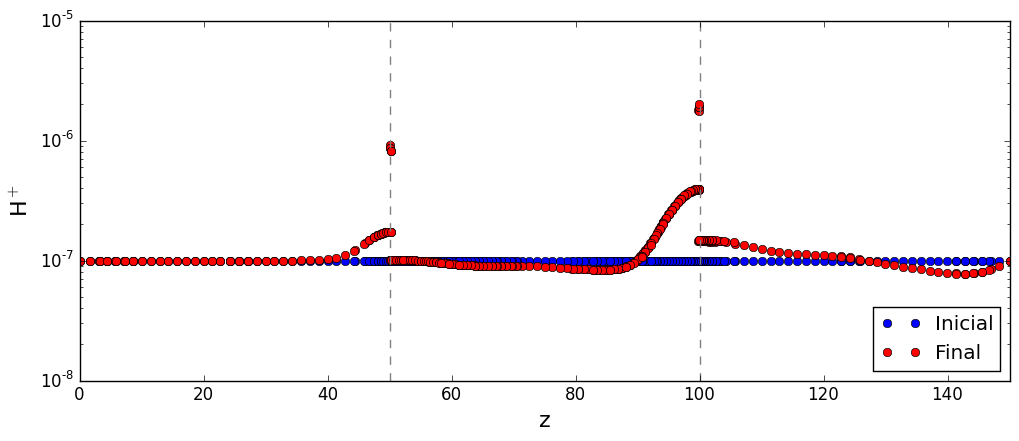
\includegraphics[width=\textwidth]{acoplado/1p160kvm/H-399}
    \caption{Concentración molar de \h{} en la curva de nivel $r = 2.5$ \si{\micro\metre}}
    \label{fig:curva-aco-h}
\end{figure}

\begin{figure}
    \centering
    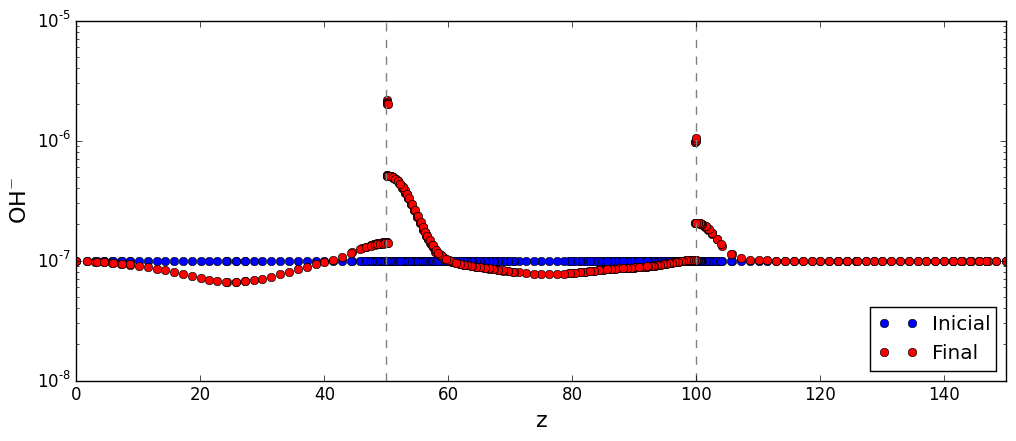
\includegraphics[width=\textwidth]{acoplado/1p160kvm/OH-399}
    \caption{Concentración molar de \oh{} en la curva de nivel $r = 2.5$ \si{\micro\metre}}
    \label{fig:curva-aco-oh}
\end{figure}

\begin{figure}
    \centering
    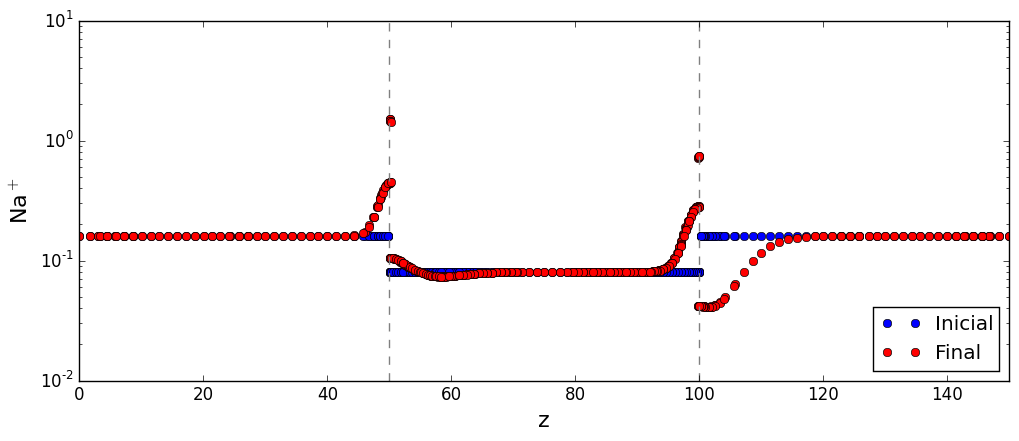
\includegraphics[width=\textwidth]{acoplado/1p160kvm/Na-399}
    \caption{Concentración molar de \na{} en la curva de nivel $r = 2.5$ \si{\micro\metre}}
    \label{fig:curva-aco-na}
\end{figure}

\begin{figure}
    \centering
    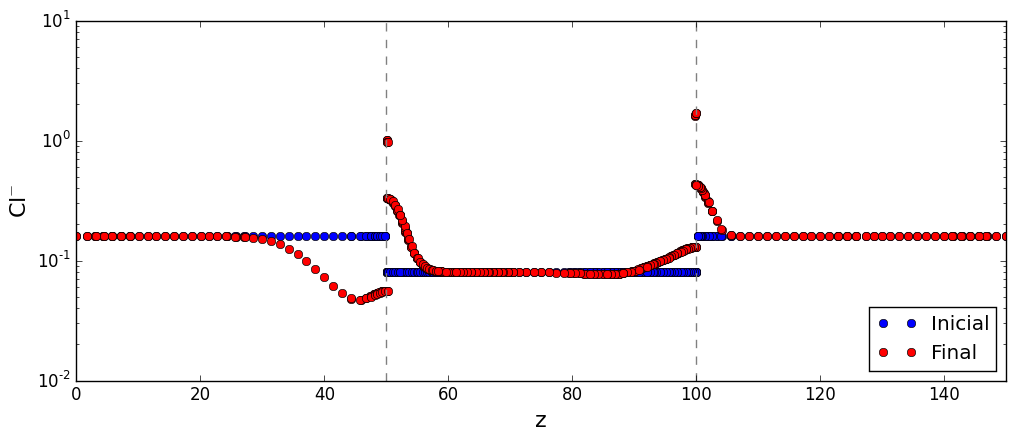
\includegraphics[width=\textwidth]{acoplado/1p160kvm/Cl-399}
    \caption{Concentración molar de \cl{} en la curva de nivel $r = 2.5$ \si{\micro\metre}}
    \label{fig:curva-aco-cl}
\end{figure}

\clearpage


\chapter{Conclusiones}

En su estado actual, el código desarrollado permite resolver sobre un dominio bidimensional que contempla simetría de revolución sobre el potencial en la membrana celular y el líquido intra y extracelular. Así mismo provee la respuesta dinámica de la creación y evolución de la población de poros de la membrana a dicho potencial aplicado. Por último analiza el transporte de cuatro especie iónicas a través de la membrana.

El modelo discretiza la membrana explícitamente, utilizando un mallado adaptativo. Debemos destacar que este modo de simular el problema es inédito ya que hasta el momento es usual en la literatura utilizar dos medios (que corresponden al líquido intra y extracelular) y considerar a la membrana como una condición de contorno sobre la que se supone un potencial PTM. Al discretizar explícitamente la membrana con elementos finitos en lugar de condiciones de contorno se obtuvieron resultados que se acercan más a la realidad. Nuestro modelo, a partir de la distribución de potencial y campo eléctrico sobre el dominio, reproduce adecuadamente tanto la forma como la magnitud del PTM. También predice correctamente el valor umbral de intensidad de pulso, más allá del cual no varía apreciablemente el PTM.

El mallado de elementos finitos seleccionado para realizar los cálculos es óptimo, pues combina un grado de precisión adecuado con estabilidad numérica. Siempre es posible extender el numero de elementos y nodos con lo cual se aumentaría el tamaño de los sistema lineales a resolver, y con ello el tiempo de cómputo. Sin embargo no obtendríamos con ello en nuestra configuración de parámetros un aumento significativo en la calidad de los resultados.

En cuanto al modelado de la dinámica y creación de la población de poros, se comprobó que la evolución de la densidad de poros es la adecuada para explicar la existencia de este umbral y que el potencial aplicado influye en la velocidad de la evolución tanto de la densidad como del radio de los poros. 
Es necesario observar que la mayoría de los poros creados se sellan muy rápidamente por lo que no influyen en el ingreso o egreso de iones dentro de la célula, por lo que si se pretende permeabilizar la membrana para las especies estudiadas, se vuelve esencial repetir el pulso periódicamente. 

El transporte de especies a través de la membrana dado por mecanismos guiados por la difusión y la movilidad de las especies iónicas responde adecuadamente a la aplicación de pulsos equi-espaciados temporalmente, observándose que la reapertura de los poros permite el reingreso de material dentro de la célula. Estos resultados responden cualitativamente a los medidos experimentalmente.

Se observaron resultados de movilidad de las especies iónicas muy diferentes entre las simulaciones que no consideraron la generación de poros en la membrana y las que sí la consideraron. Esto sirve para confirmar el efecto positivo que tiene la electroporación en el ingreso y egreso de especies a la célula.

Hay muchos tipos de análisis que quedaron pendientes y que podrían ser realizados en trabajos futuros. Entre ellos se destaca una mayor parametrización de las múltiples variables involucradas; sobre todo los pulsos eléctricos. Es posible analizar diferentes tipos de pulsos, de mayor o menor frecuencia, con potenciales más variados, con diferentes relaciones entre los tiempos de apagado y prendido y diferentes tipos de ondas. También se podría analizar de qué manera una célula puede bloquear el ingreso de especies a otra célula, o reducir el efecto de electroporación. Para esto sería necesario simular un dominio con más de una célula, lo cuál se puede realizar con facilidad con el código implementado. Al acoplar los distintos fenómenos físicos estudiados se consideró el efecto del campo eléctrico sobre la permeabilización de la membrana y sobre las concentraciones de especies, y el efecto de la permeabilización sobre las concentraciones. Un estudio más profundo de este problema debería considerar la no linealidad de la conductividad eléctrica de los tres medios considerados; esta conductividad puede depender de la concentración de especies iónicas, especialmente del pH del medio.

Otros tipos de análisis pendientes requerirían en cambio un mayor trabajo. Uno de estos tipos de análisis es el modelado de células con formas irregulares, como es comúnmente el caso en los tejidos. Esto obligaría a trabajar con un sistema de coordenadas tridimensional, dado que las células irregulares no son sólidos de revolución y no se podría aprovechar el sistema de coordenadas cilíndricas. De esta manera sería necesario reescribir gran parte del código implementado y optimizar los métodos numéricos, ya que la cantidad de elementos en la malla se incrementaría al trabajar en tres dimensiones. Por último se podría analizar también la deformación celular producida por la diferencia de potencial y se podrían modelar las organelas internas de la célula para obtener un modelo más realista.


%\appendix
%\chapter{Instrucciones de uso del código} \label{chap:uso}

\chapter{Apéndices} \label{chap:uso}

\section*{Instrucciones de uso del código}

El código entregado se puede compilar en Visual Studio importando la solución con el archivo \texttt{celula.sln}, que usa el compilador Visual C++. Se puede compilar y correr en Linux con el compilador GCC usando el archivo \texttt{Makefile}. Para compilar con Intel C Compiler es necesario modificar el \texttt{Makefile} o el proyecto de Visual Studio. Adicionalmente también se incluyen varios scripts en lenguaje Python para ayudar al proceso de generar de mallas, procesar las salidas obtenidas y generar gráficos.

\subsection*{Parámetros de entrada}

El programa recibe los parámetros de entrada a través de un archivo \texttt{input.in}, que consta de varias líneas con información de la corrida en la forma 2\texttt{parámetro: valor} donde los parámetros son los siguientes:

\begin{description}
	\item[\texttt{malla}] ruta del archivo con la malla que representa el dominio. 
	\item[\texttt{nodpel}] cantidad de nodos por elemento. La mayor parte del código solo puede correr con elementos de 4 nodos, pero el sub-problema del potencial eléctrico también puede ser ejecutado con elementos de 3 nodos.
	\item[\texttt{problema}] tipo de problema a correr. Puede ser \texttt{potencial} si solo se desean obtener los resultados de potencial eléctrico (capítulo \ref{chap:itv}), \texttt{poros} si se desea resolver el potencial y el crecimiento de poros (capítulo \ref{chap:poros}), \texttt{transporte} si se desea resolver el potencial y transporte de especies sin poros (capítulo \ref{chap:trans}) y \texttt{acoplado} si se desean correr el modelo acoplado con todos los subproblemas (capítulo \ref{chap:acoplado}).
	\item[\texttt{salida}] ruta al directorio de salida. El programa no ejecuta si el directorio de salida no está vacío (para evitar sobrescribir resultados).
	\item[\texttt{threads}] cantidad de hilos de procesamiento a utilizar. Se recomienda usar tantos como tenga el procesador.
	\item[\texttt{delta\_t}] intervalo temporal usado para el cálculo de densidad y radio de poros. Las demás ecuaciones se resuelven con intervalos temporales mayores, que son múltiplos del intervalo de poros. Si sólo se calcula el potencial eléctrico este valor se ignora. Para los resultados de este trabajo se utilizó un valor de 1 \si{\nano\second}.
	\item[\texttt{sigint}] valor de conductividad eléctrica en el interior de la célula, expresado en \si{\siemens \per \micro\metre}.
	\item[\texttt{sigext}] valor de conductividad eléctrica del líquido extracelular, expresado en \si{\siemens \per \micro\metre}.
	\item[\texttt{sigint}] valor de conductividad eléctrica en el la membrana celular, expresado en \si{\siemens \per \micro\metre}.
	\item[\texttt{potencial}] diferencia de potencial entre los electrodos, medida en \si{\volt}. Se asume que se encuentra el electrodo positivo en el borde superior de la malla y el negativo en el borde inferior.
	\item[\texttt{radio}] radio de la célula, medido en \si{\micro\metre}.
	\item[\texttt{ancho}] ancho de la membrana celular, medido en \si{\micro\metre}.
	\item[\texttt{pulsos}] cantidad de pulsos a simular.
	\item[\texttt{on\_time}] tiempo que estará prendido cada uno de los pulsos, medido en segundos.
	\item[\texttt{off\_time}] tiempo que estará apagado cada uno de los pulsos, medido en segundos. 
\end{description}

Los parámetros pueden estar en cualquier orden y puede haber en el archivo \texttt{input.in} comentarios que comiencen con \texttt{\#}. La malla del dominio debe ser un archivo de texto con el siguiente formato:

\begin{itemize}
	\item Una línea con la cantidad de nodos.
	\item Una línea con cada nodo indicando el número de nodo y las posiciones en $x$ e $y$ separados por espacios.
	\item Una línea con la cantidad de zonas del dominio.
	\item Una línea por cada zona del dominio, con un número de zona y la cantidad de elementos de la zona, separados por espacios.
	\item Una línea por cada elemento de cada zona, con un número de elemento dentro de la zona y los números de los nodos que componen el elemento, separados por espacios.
\end{itemize}

\subsection*{Formatos de salida}

El programa genera varias carpetas y archivos en el directorio de salida indicado:

\begin{itemize}
	\item En el directorio \texttt{tension} genera cada 100\usec de la simulación archivos con el nombre \texttt{tension.csv.xxx} con \texttt{xxx} números consecutivos. Los archivos tienen valores de potencial eléctrico para cada nodo, indicado con coordenadas $x$ e $y$.
	\item En el directorio \texttt{campo} genera cada 100\usec archivos con nombre \texttt{campo.csv.xxx} con valores de las componentes horizontal y vertical y módulo del campo eléctrico y valores de corriente de cada elemento, indicado con coordenadas $x$ e $y$.
	\item En el directorio \texttt{poros} genera archivos con nombre \texttt{posos.csv.xxx} cada 100\usec con el ángulo polar y el radio en \um de cada poro de la membrana. 
	\item En el directorio \texttt{concentracion} genera archivos \texttt{concentracion.csv.xxx} cada 100\usec con los valores de concentración de \h, \oh, \na y \cl en cada nodo expresados en átomos por \si{\micro\metre\cubed}.
	\item En el directorio \texttt{concentracion} genera archivos \texttt{molar.csv.xxx} con los mismos valores de concentración pero expresados como concentraciones molares.
	\item En el directorio \texttt{concentracion} genera archivos con los valores de pH y pOH de cada nodo.
	\item En un único archivo \texttt{itv.csv} graba periódicamente valores de potencial transmembrana indicados con columnas de tiempo, ángulo polar y PTM.
	\item Genera una copia del archivo \texttt{input.in} utilizado.
\end{itemize}

%esto mejor no poner: por salida se imprimen periodicamente el tiempo de la simulación, el error en el cálculo de transporte, la cantidad de poros, y el tiempo por iter en promedio


\backmatter
\bibliography{tesis}

\begin{thebibliography}{99}

%TODO agregar títulos a los que les falta!!
%TODO poner nombres en lugar de iniciales

\bibitem{c1}
	Colombo L., González G., Marshall G., Molina F., Soba A., Suárez C., Turjanski P.
	Bioelectrochemistry 71,
	2007

\bibitem{c2}
	Nilsson E, von Euler H, Berendson J, Thorne A, Wersall P, Naslund I, Lagerstedt A, Narfstrom K, Olsson J
	Bioelectrochemistry 51,
	2000

\bibitem{c3}
	Netti PA, Berk DA, Swartz MA, Grodzinsky AJ, Jain RK
	Cancer Research 60,
	2000

\bibitem{c4}
	Matías Daniel Marino, Dr. Pablo Turjanski, Dr. Nahuel Olaiz
	\emph{Electroporación en el tratamiento de tumores: modelos teóricos y experimentales}
	2013

\bibitem{c5}
	G. Puchiar, T. Kotnik, B. Valic and D. Miklavcic
	\emph{FALTA EL NOMBRE!!!}
	Annals of Biomedical Engineering
	Volume 34, 4, 2006

\bibitem{c6-fodava}	
	Qiong Zheng, Duan Chen, Guo-Wei Wei
	\emph{FALTA EL NOMBRE!!!}
	Journal of Computational Physics,	
	Volume 230, 13, 2011

\bibitem{c7-krass07}	
	Wanda Krassowska, Petar D. Filev,
	\emph{FALTA EL NOMBRE!!!}
	Biophysical Journal, Volume 92, Issue 2, 2007

\bibitem{c8}
	Jianbo Li, Hao Lin
	\emph{Numerical simulation of molecular uptake via electroporation}
	Bioelectrochemistry 82, 10–21, 2011 

\bibitem{c9-fem-electro}
	Stanley Humphries
	\emph{Finite-element Methods for Electromagnetics}
	2010

\bibitem{c10}
	O.C. Zienkiewicz, R.L. Taylor
	\emph{The Finite Element Method Volume I: The Basis}
	Butterworth-Heinemann, 5th edition, 2000

\bibitem{c11}
	\emph{Automesh 2D}
	\texttt{http://www.automesh2d.com/}

\bibitem{c12}
	Geoffrey M. Cooper, Robert E. Hausman
	\emph{La Célula}
	2$^{\circ}$ edición, 
	Marbán

\bibitem{c13}	
	P.H. Mott, J.R. Dorgan, C.M. Roland 
	\emph{The bulk modulus and Poisson's ratio of incompressible materials} 
	Journal of Sound and Vibration 312, 572–575, 2008
	
\bibitem{c14}
	John David Jackson
	\emph{Classical Electrodynamics}
	3$^{\circ}$ edición,
	John Wiley \& Sons Inc.,
	1999

\bibitem{c15}	
	Antonio Nives
	\emph{Métodos numéricos aplicados a la ingeniería}
	Grupo editorial Patria,
	2007

\bibitem{c16}
	\emph{Paraview}
	\texttt{www.paraview.org}
	Sandia National Laboratory, Kitware Inc, Los Alamos National Laboratory

\bibitem{matplotlib}
	\emph{matplotlib}
	\texttt{http://matplotlib.org/}
	

%\bibitem{krass}
%	Wanda Krassowska and Petar D. Filev
%	\emph{Modeling Electroporation in a Single Cell}
%	Biophysical Journal
%	Volume 92, Issue 2, 15 January 2007, Pages 404–417

\bibitem{tsong}
	Tsong, T. Y.
	\emph{Electroporation of cell membranes}
	Biophys. J. 60:297–306, 1991

\bibitem{krass-viejo}
	Katherine A. DeBruin, Wanda Krassowska, 
	\emph{Modeling Electroporation in a Single Cell. I. Effects of Field Strength and
Rest Potential}
	Biophysical Journal, Volume 77, 1999
	
\bibitem{eigen}
	\emph{Eigen}
	\texttt{http://eigen.tuxfamily.org/}
	
\bibitem{burden}
	Richard L. Burden, J. Douglas Feires
	\emph{Análisis numérico}
	Séptima edición, I.T.P. Latin America, 2001

\bibitem{yousef}
	Yousef Saad
	\emph{Iterative Methods for Sparse Linear Systems}
	Seguna edición, Society for Industrial and Applied Mathematics, 2003
	
\end{thebibliography}


\end{document}
